% !TEX root = main.tex

\documentclass[12pt,a4paper]{article}
\usepackage{graphicx} % For including images
\usepackage{microtype}
\usepackage{enumitem}
\usepackage{geometry} % Adjust page margins
\usepackage{setspace} % For line spacing
\usepackage{titlesec} % For section formatting
\usepackage{tocloft} % For TOC formatting
\usepackage{float}  % allows H specifier
\usepackage{placeins} % \FloatBarrier to stop floats crossing section boundaries
\usepackage{silence}
\usepackage{amsmath}
\usepackage[backend=biber,style=ieee]{biblatex}
\usepackage{pgfgantt} % put in preamble
\addbibresource{references/intro.bib}
\addbibresource{references/literature_review.bib}
\addbibresource{references/vio_algorithms.bib}
\addbibresource{references/methodology.bib}


% Page setup
\geometry{margin=1in}
\setstretch{1.3} % Line spacing
\setlength{\emergencystretch}{3em} % reduce overfull \hbox warnings
\hbadness=10000 % suppress underfull \hbox warnings
\hfuzz=20pt % ignore overfull \hbox warnings up to 20pt


\title{
{\Huge \textbf{Progress Report}} \\[1cm]
\textbf{Visual-Inertial Navigation \\ 
for Autonomous UAV Operation \\ 
in GPS-Restricted Environments}
\vspace{4cm}
}


\author{
\textbf{Project Supervisors - Internal:} \\
Prof. Chandana Gamage \\
\\
\textbf{Group Members:} \\
\begin{tabular}{l l} % Two columns, left-aligned, no borders
D. V. A. I. Delgahagoda & 210113L \\
T. T. Kashmeera & 210279A \\
K. D. R. P. Rathnayake & 210537N \\
\end{tabular}
\vspace{4cm}
}
\date{} 
\begin{document}

\maketitle
\begin{center}
Department of Computer Science and Engineering \\
University of Moratuwa
\end{center}
\thispagestyle{empty} % No page number on title page

\newpage
\renewcommand{\contentsname}{\Large \textbf{Table of Content}}
\tableofcontents
\thispagestyle{empty}

\newpage
\renewcommand{\listfigurename}{\Large \textbf{Table of Figures}}
\listoffigures
\thispagestyle{empty} % Optional: no page number on this page

\newpage
\setcounter{page}{1} % Start numbering from here

\section{Introduction}

\subsection{Overview}

Unmanned Aerial Vehicles (UAVs), commonly referred to as drones, have rapidly expanded their role across a wide range of applications including aerial mapping, infrastructure inspection, environmental monitoring, surveillance, and autonomous delivery \cite{ref1,ref2}. Their ability to operate in remote, hazardous, or inaccessible environments makes them valuable tools for both civilian and industrial use. As UAV deployments increase in complexity, the demand for reliable autonomous navigation capabilities has become increasingly critical.

A fundamental requirement for autonomous UAV operation is accurate and continuous localization, which enables the UAV to estimate its position and orientation in space. Reliable localization is essential for trajectory tracking, obstacle avoidance, flight stabilization, and mission execution. Without accurate localization, UAV autonomy is severely limited, restricting operations to controlled or manually supervised environments \cite{ref3}.

The Global Positioning System (GPS) is currently the primary localization method used in UAV systems due to its ability to provide global position information with reasonable accuracy. However, GPS-based navigation has significant limitations in environments where satellite signals are weak, obstructed, or unavailable. These limitations restrict UAV deployment in many real-world scenarios and highlight the need for alternative onboard localization solutions capable of operating independently of external positioning infrastructure.

Advancements in onboard sensing and perception technologies, particularly camera and inertial sensors, have enabled the development of autonomous localization methods that do not rely on GPS. These methods allow UAVs to estimate their motion and position using onboard sensor data, enabling reliable navigation in GPS-denied environments and expanding the operational capabilities of autonomous aerial systems.

\subsection{Problem Statement}

Reliable localization is a fundamental requirement for autonomous UAV navigation. Most UAV systems rely heavily on the Global Positioning System (GPS) to obtain position information for navigation and control. While GPS performs effectively in open outdoor environments, its reliability significantly degrades or becomes completely unavailable in GPS-denied environments such as indoor spaces, dense urban areas, underground environments, and regions with heavy signal obstruction \cite{ref6,ref7}.

In urban environments, tall structures obstruct satellite line-of-sight and introduce multipath effects, resulting in large positioning errors. Indoor and underground environments completely block GPS signals, making satellite-based localization impossible. Similarly, environments such as forests or industrial facilities introduce signal attenuation and interference that further reduce positioning reliability.

\begin{figure}[H]
    \centering
    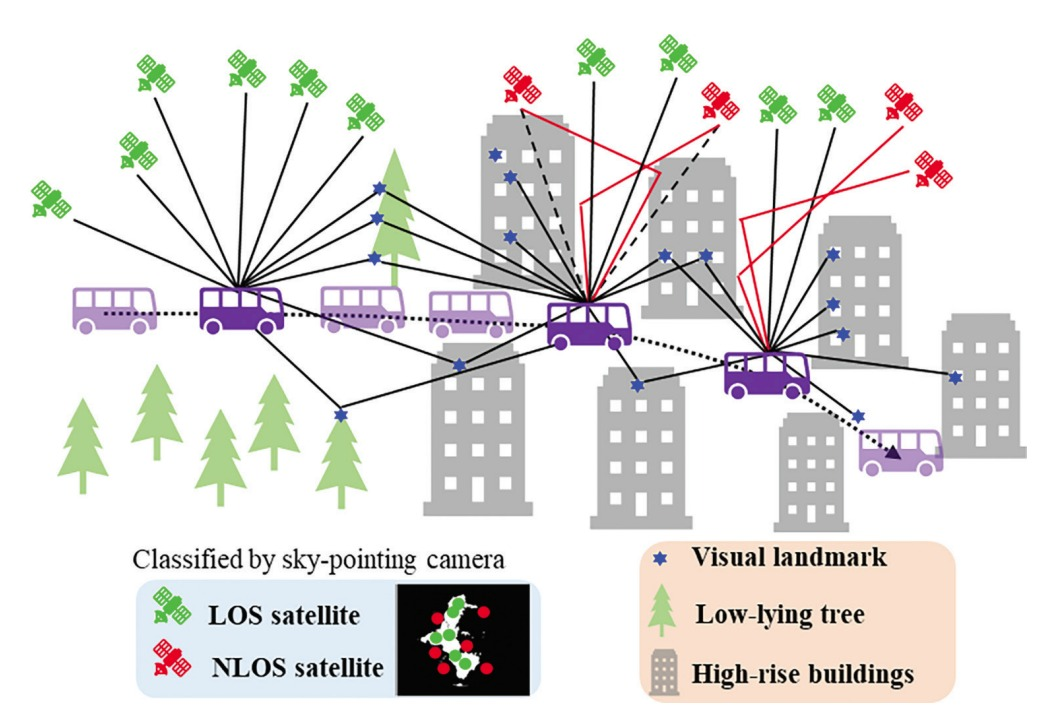
\includegraphics[width=0.8\textwidth]{images/gnss_signal.jpg}
    \caption{GNSS signal classification with LOS/NLOS satellites and visual landmarks in urban environments \cite{imgref1}.}
    \label{fig:gnss}
\end{figure}

The loss or degradation of GPS signals severely affects UAV navigation performance, leading to inaccurate positioning, trajectory deviations, and potential mission failure. These limitations prevent UAVs from operating autonomously in many real-world environments where GPS is unreliable or unavailable. Therefore, there is a critical need for reliable onboard localization methods that enable autonomous UAV navigation in GPS-denied environments without relying on satellite-based positioning systems.

\subsection{Research Objectives}

The main objective of this project is to develop and improve a robust localization system to enable autonomous UAV navigation in GPS-denied environments using onboard sensing technologies.

The specific objectives of this research are as follows:

\begin{itemize}

\item Study and analyze existing localization methods for UAV navigation in GPS-denied environments.

\item Evaluate alternative onboard localization approaches and select a suitable method for autonomous UAV operation.

\item Analyze existing Visual SLAM and Visual-Inertial SLAM algorithms and select an appropriate model for implementation.

\item Implement the selected localization model on a UAV platform and evaluate its baseline localization performance.

\item Identify limitations and performance constraints of the implemented system under real-world operating conditions.

\item Develop and integrate deep learning-based improvements to enhance localization robustness and accuracy.

\item Evaluate and compare the performance of the improved system against the baseline implementation.

\end{itemize}

\subsection{Purpose and Scope of the Project}

This project focuses on the development and evaluation of a robust onboard localization system for autonomous UAV operation in GPS-denied environments. The scope of the project includes the analysis of existing localization methods, selection and implementation of a suitable Visual-Inertial SLAM model, and evaluation of its performance on a UAV platform.

Furthermore, this project aims to investigate the limitations of the selected model and explore deep learning-based techniques to improve localization robustness and accuracy. The final outcome is a UAV system capable of reliable autonomous navigation using onboard visual and inertial sensing without dependence on GPS, enabling operation in challenging and previously inaccessible environments.
\section{Literature Review}
\sloppy

This review begins by examining popular navigation methods for UAV operation in GPS-restricted environments, comparing their sensing principles, estimation strategies, and operational trade-offs. It then presents the fundamentals of VINS, covering sensor characteristics (camera/IMU), common fusion architectures (loosely vs. tightly coupled), back-end estimation (filtering vs. optimization), and representative geometric and learning-based systems used in practice.

\subsection{Navigation Methods for UAVs in GPS-Denied Environments}

Reliable navigation in GPS-denied environments is critical for autonomous UAV operation. Several sensing and estimation approaches have been developed, each offering different trade-offs in accuracy, robustness, computational complexity, and hardware requirements.

\subsubsection{Visual-Inertial Navigation Systems (VINS)}

Visual--Inertial Navigation Systems (VINS) tightly fuse camera and IMU measurements within a nonlinear optimization or filtering framework. The IMU provides high-rate motion propagation, while visual observations reduce drift through feature tracking and bundle adjustment. Modern approaches often employ sliding-window optimization or factor graph methods.

VINS provides accurate 6-DoF pose estimation, real-time capability, and independence from external infrastructure, making it well suited for UAV navigation in GPS-denied environments \cite{qin2018vins, forster2017manifold, cadena2016slam}. However, performance depends on sufficient visual texture and computational resources.

\subsubsection{LiDAR-Based Navigation}

LiDAR-based navigation estimates UAV pose by registering three-dimensional point clouds. These systems are robust to illumination variations and provide strong geometric consistency. When fused with inertial sensors, LiDAR systems achieve improved robustness and long-term accuracy.

Despite their precision, LiDAR sensors increase payload weight, power consumption, and system cost, which may limit their application in lightweight UAV platforms \cite{zhang2014loam, shan2018lego}.

\subsubsection{Dead Reckoning and Pure Inertial Navigation}

Dead reckoning estimates position by integrating motion measurements over time, typically using IMU data. Inertial navigation systems offer high update rates and short-term accuracy; however, errors accumulate rapidly due to sensor bias and noise. Consequently, pure inertial navigation is unsuitable for long-duration autonomous flight without external correction \cite{titterton2004strapdown}.

\subsubsection{Optical Flow-Based Navigation}

Optical flow-based navigation estimates relative motion by tracking pixel displacement between consecutive image frames. These methods are computationally efficient and lightweight, making them attractive for small UAV platforms. However, they primarily provide velocity estimates and suffer from drift over time. Performance is also sensitive to lighting conditions and surface texture \cite{scaramuzza2014vision}.

\subsubsection{Beacon-Based Navigation}

Beacon-based navigation systems, such as Ultra-Wideband (UWB) positioning, estimate location relative to fixed anchors using time-of-flight measurements. These systems can achieve high indoor accuracy but require pre-installed infrastructure and are geographically constrained \cite{ledergerber2015robot}.

\subsubsection{Summary}
\begin{table}[H]
\centering
\caption{Comparison of UAV Navigation Methods in GPS-Denied Environments}
\label{tab:uav_navigation_methods}
\begin{tabular}{|p{3cm}|p{4.2cm}|p{4.2cm}|p{3.4cm}|}
\hline
\textbf{Method} & \textbf{Key Principle} & \textbf{Strengths} & \textbf{Limitations} \\
\hline
Visual--Inertial Navigation (VINS) & Fuses camera and IMU in an optimization or filtering framework. & Accurate 6-DoF pose, real-time capable, no external infrastructure. & Requires visual texture and adequate compute. \\
\hline
LiDAR-Based Navigation & Registers 3D point clouds, often fused with IMU. & Strong geometric consistency, robust to lighting. & Higher payload, power, and cost. \\
\hline
Dead Reckoning / Pure Inertial & Integrates IMU measurements to estimate motion. & High update rate, simple sensing stack. & Rapid drift from bias and noise. \\
\hline
Optical Flow & Tracks pixel motion between frames for relative motion. & Lightweight, computationally efficient. & Primarily velocity estimates; drift, sensitive to lighting/texture. \\
\hline
Beacon-Based Navigation (e.g., UWB) & Ranges to fixed anchors for positioning. & High indoor accuracy. & Requires installed infrastructure; limited coverage. \\
\hline
\end{tabular}
\end{table}

\subsubsection{Justification for Choosing Visual-Inertial Navigation}
After comparing navigation methods for GPS-denied environments, Visual--Inertial Navigation Systems (VINS) were selected as the primary approach for this project.
\begin{itemize}
    \item Provides accurate 6-DoF pose estimation without external infrastructure.
    \item Balances robustness and hardware feasibility for UAV platforms.
    \item Leverages complementary camera and IMU sensing to reduce drift.
    \item Supports real-time operation with established optimization and filtering pipelines.
\end{itemize}


\subsection{Overview of Visual Inertial Navigation}
A comprehensive understanding of Visual–Inertial Navigation Systems (VINS) requires analyzing both their sensor foundations and estimation architectures. VINS performance is fundamentally constrained by the quality of IMU and visual measurements and the accuracy of their error models. MEMS-based IMUs, widely used in UAVs due to favorable SWaP-C characteristics, measure specific force and angular velocity using accelerometers and gyroscopes \cite{ref21}. However, their outputs are affected by bias, scale factor errors, and stochastic noise, which must be modeled and estimated online to prevent rapid drift \cite{ref21,ref23,ref24}. To ensure computational feasibility in tightly-coupled frameworks, IMU pre-integration combines high-rate inertial measurements between camera frames into efficient motion constraints \cite{ref20}. On the visual side, monocular configurations offer low cost and weight but cannot directly observe absolute scale without inertial fusion \cite{ref26,ref27}, whereas stereo setups provide immediate depth and metric scale at the expense of higher complexity and calibration requirements \cite{ref25,ref27}. Architecturally, tightly-coupled fusion—where raw visual and inertial data are jointly estimated—offers superior accuracy and robustness compared to loosely-coupled approaches \cite{ref28,ref29,ref30}. For state estimation, filtering methods such as the EKF provide computational efficiency but suffer from linearization-induced inconsistency \cite{openvins,orbslam3,cuvslam}, while optimization-based (smoothing) approaches, typically implemented with sliding-window nonlinear least squares, achieve higher accuracy by jointly minimizing visual and inertial residuals over multiple states \cite{ref30,openvins,qvio}.

\subsection{Visual SLAM for UAV Navigation}

Simultaneous Localization and Mapping (SLAM) is a fundamental technique in robotics that enables a robot or UAV to build a map of an unknown environment while estimating its own pose within that map. When the primary sensing modality is a camera, the process is referred to as Visual SLAM (V-SLAM).

\subsubsection{Core Concept}

Visual SLAM relies on detecting and tracking visual features across consecutive camera frames. These features, often keypoints or corners, are used to estimate the relative motion of the UAV. By accumulating these measurements, the system can reconstruct a map and simultaneously localize itself in 3D space.

Modern V-SLAM algorithms often integrate multiple components:

\begin{itemize}
    \item \textbf{Feature Extraction and Tracking:} Identify salient points in each frame and match them across frames.
    \item \textbf{Pose Estimation:} Compute the UAV’s camera motion based on the observed feature correspondences.
    \item \textbf{Map Optimization:} Refine both UAV poses and 3D feature positions using techniques such as bundle adjustment or graph optimization.
    \item \textbf{Loop Closure:} Detect when the UAV revisits previously mapped areas and correct accumulated drift.
\end{itemize}

\subsubsection{Applications in UAVs}

Visual SLAM provides accurate 6-DoF pose estimates without relying on external signals, making it suitable for GPS-denied environments. It can operate with monocular, stereo, or RGB-D cameras and is often combined with inertial measurements in VINS frameworks for improved robustness \cite{qin2018vins, forster2017manifold, cadena2016slam}.

\subsubsection{Advantages and Limitations}

\textbf{Advantages:}
\begin{itemize}
    \item Operates independently of GNSS infrastructure.
    \item Can provide dense or sparse 3D mapping for navigation and planning.
    \item Compatible with lightweight UAV platforms using only cameras.
\end{itemize}

\textbf{Limitations:}
\begin{itemize}
    \item Performance depends on sufficient visual texture and lighting conditions.
    \item Sensitive to motion blur and dynamic scenes.
    \item Computationally demanding, especially for real-time, large-scale mapping.
\end{itemize}

\subsection{A Review of VIO/VSLAM Models}
This section reviews classical vision technique-based VIO/VSLAM models, focusing on established pipelines that rely on feature extraction, geometric constraints, and optimization or filtering to estimate motion and map structure.

\subsubsection{openVINS}
OpenVINS (Open Visual-Inertial Navigation System) is an open-source, filter-based visual–inertial odometry (VIO) framework developed for real-time state estimation in robotics, UAVs, and AR/VR applications. The system is built upon the Multi-State Constraint Kalman Filter (MSCKF) framework, where the state vector consists of IMU pose, velocity, inertial biases, and a sliding window of historical camera poses. Instead of explicitly estimating 3D landmarks, OpenVINS leverages multi-view feature constraints to update the state efficiently[1]. High-rate IMU measurements are used for state propagation, while visual measurements are incorporated through feature tracking (typically KLT optical flow) and RANSAC-based outlier rejection. The framework is implemented in modern C++ with ROS integration, OpenCV for image processing, and Eigen for linear algebra operations. Experimental evaluations on datasets such as EuRoC MAV demonstrate competitive accuracy with low translational drift (approximately 1–3\%)\cite{openvins} while maintaining real-time performance on CPU-only systems.

\noindent\textbf{Advantages:} Efficient MSCKF filtering enables real-time, CPU-only deployment; the pipeline is modular and supports online camera--IMU extrinsic and time-offset calibration.

\noindent\textbf{Disadvantages:} No built-in loop closure or persistent mapping, so drift accumulates over long trajectories; performance depends on reliable feature tracking and degrades in low-texture or visually degraded scenes.

\subsubsection{ORB-SLAM3}
ORB-SLAM3 is a state-of-the-art, open-source visual (and visual–inertial) simultaneous localization and mapping (SLAM) system designed for accurate and globally consistent pose estimation in robotics, AR/VR, and autonomous navigation applications. It extends the ORB-SLAM family by supporting monocular, stereo, RGB-D, and visual–inertial configurations within a unified framework\cite{orbslam3}. The system follows a keyframe-based, optimization-driven architecture built around ORB (Oriented FAST and Rotated BRIEF) features for robust and efficient feature extraction and matching.
The core architecture consists of three parallel threads: Tracking, Local Mapping, and Loop Closing. The Tracking thread extracts ORB features, estimates camera pose via motion models and Perspective-n-Point (PnP) optimization, and decides keyframe insertion. The Local Mapping thread performs local bundle adjustment (BA) to optimize poses and 3D landmarks within a sliding window of keyframes. The Loop Closing thread detects place revisits using bag-of-words (BoW) place recognition and performs pose graph optimization and full bundle adjustment to ensure global consistency.
In visual–inertial mode, ORB-SLAM3 tightly integrates IMU measurements using preintegration theory and performs joint optimization over visual and inertial states. The system is implemented in C++ and relies on OpenCV for image processing, Eigen for linear algebra, DBoW2 for place recognition, and g2o for nonlinear graph optimization. Evaluations on benchmark datasets such as EuRoC MAV and TUM-VI demonstrate high accuracy with strong global consistency, often outperforming previous ORB-SLAM versions and many contemporary SLAM systems.

\begin{figure}[H]
    \centering
    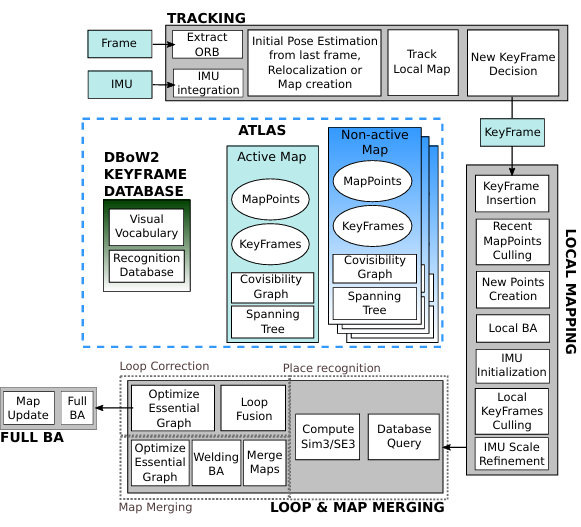
\includegraphics[width=0.8\textwidth]{images/orbslam3.png}
    \caption{ORB-SLAM3 Architecture \cite{orbslam3}.}
    \label{fig:orblsma3_architecture}
\end{figure}

\begin{itemize}
    \item \textbf{Advantages:} ORB-SLAM3 achieves high global accuracy by combining robust place recognition with loop closing and full bundle adjustment, which significantly reduces drift over long trajectories. It supports monocular, stereo, RGB-D, and tightly coupled visual--inertial configurations and maintains a persistent, reusable map for long-term and multi-session localization.
    \item \textbf{Disadvantages:} Its optimization-heavy pipeline (bundle adjustment and pose-graph optimization) increases CPU and memory requirements relative to filter-based systems, and the multi-threaded architecture adds implementation and tuning complexity. Additionally, monocular and visual--inertial initialization can be sensitive to motion conditions, making early-stage tracking less reliable in some scenarios.
\end{itemize}

\subsubsection{PyCuVSLAM}
PyCuVSLAM is a Python interface for the CUDA‑accelerated visual SLAM (cuVSLAM) library developed by NVIDIA Research, providing high‑performance visual odometry and SLAM capabilities with GPU acceleration. PyCuVSLAM wraps the underlying cuVSLAM C++/CUDA implementation in a Python API, allowing real‑time processing of visual data from monocular, stereo, RGB‑D, multicamera, and visual–inertial (IMU) configurations with low latency and high throughput. The system leverages NVIDIA GPUs (via CUDA) to accelerate feature tracking, pose estimation, mapping, and loop closure tasks, making it suitable for demanding robotics, UAV, and perception applications where CPU‑only SLAM may be too slow\cite{cuvslam}. PyCuVSLAM supports ROS2 integration and example workflows for standard datasets such as EuRoC and KITTI, and produces camera pose estimates, sparse maps, and other SLAM outputs in real time. Its design emphasizes computational efficiency through parallel CUDA kernels while exposing a user‑friendly Python interface suitable for rapid prototyping and research. 

\begin{figure}[H]
    \centering
    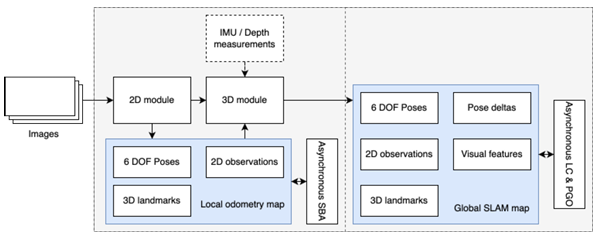
\includegraphics[width=0.8\textwidth]{images/cuvslam.png}
    \caption{cuVSLAM Architecture \cite{cuvslam}.}
    \label{fig:cuvslam_architecture}
\end{figure}

\begin{itemize}
    \item \textbf{Advantages:} CUDA acceleration enables high-throughput, low-latency SLAM that can outperform many CPU-only pipelines, while the Python API and ROS2 support simplify prototyping and integration. It supports multiple sensing setups, including RGB-D, IMU (visual--inertial), and multicamera configurations.
    \item \textbf{Disadvantages:} It depends on NVIDIA CUDA-capable GPUs and is distributed under a non-commercial NVIDIA license, limiting portability and commercial deployment. Setup can be complex due to CUDA/ROS2 dependencies, and the system has comparatively limited peer-reviewed validation (primarily an arXiv reference).
\end{itemize}

\subsubsection{Qualcomm qVIO}
 Qualcomm qVIO (Qualcomm Visual–Inertial Odometry) is a proprietary visual–inertial tracking solution developed by Qualcomm for real-time pose estimation on mobile and embedded platforms powered by Qualcomm Snapdragon processors. It is designed primarily for augmented reality (AR), virtual reality (VR), robotics, and mobile perception applications where low latency and power efficiency are critical.
qVIO performs tightly coupled fusion of camera and inertial measurement unit (IMU) data to estimate 6-DoF pose. The system leverages Qualcomm’s heterogeneous computing architecture, utilizing the CPU, GPU, and Digital Signal Processor (DSP) (e.g., Hexagon DSP) to accelerate visual feature processing and inertial fusion. The architecture typically consists of image feature extraction and tracking, IMU propagation, sensor fusion via nonlinear filtering or optimization-based methods, and drift correction mechanisms. The design emphasizes low-power real-time performance suitable for mobile SoCs rather than desktop-class systems.
qVIO has been widely used in Snapdragon-based development platforms such as Qualcomm’s Robotics RB-series and earlier AR/VR reference devices. Performance characteristics generally include low-latency tracking, robustness under moderate motion, and hardware-accelerated execution optimized for Snapdragon chipsets.\cite{qvio}

\begin{figure}[H]
    \centering
    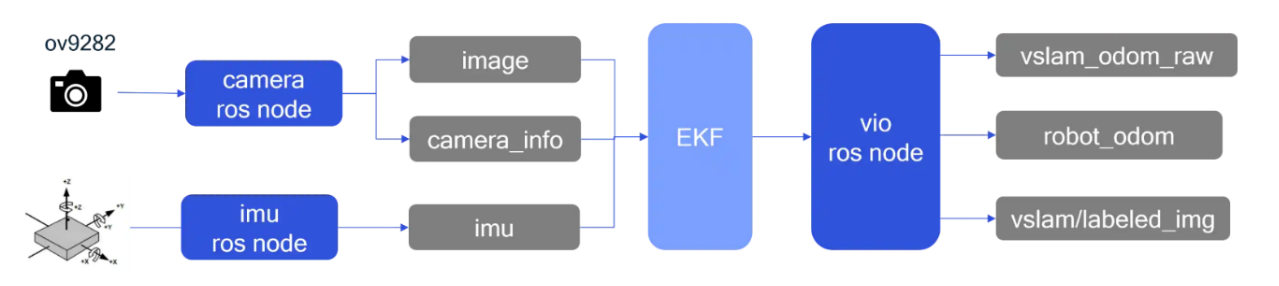
\includegraphics[width=0.8\textwidth]{images/qualcom_qvio.png}
    \caption{qVIO pipeline \cite{qvio}.}
    \label{fig:qvio_pipeline}
\end{figure}

\begin{itemize}
    \item \textbf{Advantages:} It directly mitigates the primary failure mode of traditional SLAM by robustly handling dynamic environments. This results in a significant boost in localization accuracy and system robustness in real-world scenarios, while maintaining the real-time performance of the underlying ORB-SLAM3 framework.
    \item \textbf{Disadvantages:} Its effectiveness is fundamentally limited by the capabilities of the object detector. It cannot handle moving objects that do not belong to one of its known classes, and its performance may degrade if the detector is not robust to different viewpoints or lighting conditions.
\end{itemize}

\subsubsection{Summary}

\begin{table}[H]
\centering
\scriptsize % reduces font size
\caption{Comparison of VIO Algorithms}
\resizebox{\textwidth}{!}{%
\begin{tabular}{|p{1.6cm}|p{1.9cm}|p{1.4cm}|p{1.9cm}|p{4.1cm}|p{4.1cm}|}
\hline \textbf{Algorithm} & \textbf{Core Method} & \textbf{Coupling} & \textbf{Camera Support} & \textbf{Key Innovations \& Strengths} & \textbf{Key Limitations \& Challenges} \\

\hline openVINS & Filter-based (EKF/MSCKF) & Tightly & Monocular, Stereo &
\begin{itemize}[leftmargin=*, topsep=0pt, itemsep=0pt, parsep=0pt, partopsep=0pt]
  \item Open-source, modular EKF-based VIO with MSCKF-style feature handling.
  \item Real-time on embedded platforms; flexible sensor/feature front-end.
  \item Well-suited for research comparisons and UAV implementations.
\end{itemize} &
\begin{itemize}[leftmargin=*, topsep=0pt, itemsep=0pt, parsep=0pt, partopsep=0pt]
  \item Generally lower accuracy than optimization-based smoothing methods.
  \item Requires careful tuning/calibration for best consistency.
  \item No native global map reuse/loop closure (drift over long trajectories).
\end{itemize} \\

\hline ORB-SLAM3 & Optimization-based (MAP/BA, SLAM) & Tightly & Monocular, Stereo, RGB-D &
\begin{itemize}[leftmargin=*, topsep=0pt, itemsep=0pt, parsep=0pt, partopsep=0pt]
  \item Visual--inertial SLAM with relocalization, loop closure, and multi-map (Atlas).
  \item Strong accuracy and long-term robustness for re-visitation / tracking loss.
\end{itemize} &
\begin{itemize}[leftmargin=*, topsep=0pt, itemsep=0pt, parsep=0pt, partopsep=0pt]
  \item Heavyweight SLAM system (complexity and compute) vs.\ pure odometry.
  \item Integration/tuning overhead can be high for constrained UAV stacks.
\end{itemize} \\

\hline cuVSLAM (pycuVSLAM) & GPU-accelerated VSLAM/VIO & Tightly & Mono, Stereo, RGB-D, +IMU &
\begin{itemize}[leftmargin=*, topsep=0pt, itemsep=0pt, parsep=0pt, partopsep=0pt]
  \item CUDA-accelerated pipeline enables low-latency, high-throughput tracking.
  \item Python API and ROS2 integration simplify prototyping.
  \item Supports IMU and multi-camera configurations.
\end{itemize} &
\begin{itemize}[leftmargin=*, topsep=0pt, itemsep=0pt, parsep=0pt, partopsep=0pt]
  \item Requires NVIDIA CUDA-capable GPU (portability constraints).
  \item Licensing can restrict commercial deployment.
  \item Limited peer-reviewed benchmarking relative to academic baselines.
\end{itemize} \\

\hline Qualcomm qVIO & Proprietary VIO (mobile SoC) & Tightly & Monocular (typical) &
\begin{itemize}[leftmargin=*, topsep=0pt, itemsep=0pt, parsep=0pt, partopsep=0pt]
  \item Optimized for Snapdragon platforms (CPU/GPU/DSP acceleration) with low power.
  \item Low-latency 6-DoF tracking for AR/VR and embedded robotics use.
\end{itemize} &
\begin{itemize}[leftmargin=*, topsep=0pt, itemsep=0pt, parsep=0pt, partopsep=0pt]
  \item Closed-source/proprietary; limited transparency and academic validation.
  \item Platform-locked to Qualcomm ecosystem and supported devices.
\end{itemize} \\

\hline \end{tabular}}
\label{tab:VINS_comparison}
\end{table}

\subsubsection{Justification for Choosing ORB-SLAM3}
After comparing VIO/VSLAM models, ORB-SLAM3 was selected as the primary baseline for this project.
\begin{itemize}
    \item Provides strong global consistency through loop closure and full bundle adjustment.
    \item Supports monocular, stereo, RGB-D, and visual--inertial configurations within one framework.
    \item Demonstrates high accuracy on standard benchmarks and practical UAV scenarios.
    \item Offers a mature, widely adopted open-source codebase with extensive documentation.
\end{itemize}

\subsection{A Review of Deep Learning Based VSLAM Models}
This section reviews deep learning-based improvements built on ORB-SLAM3 to understand how these additions can enhance performance and mitigate known limitations in the base system.

\subsubsection{SUPERSLAM3}
SUPERSLAM3 modifies the front-end of the ORBSLAM3 framework by replacing the traditional ORB feature extractor and BRIEF descriptor with the SuperPoint convolutional encoder-decoder architecture. To mimic ORBSLAM3's multi-scale approach, the system scales the input grayscale image to multiple pyramid levels and processes each independently through the SuperPoint network. Instead of using image sub-block division, SUPERSLAM3 selects a defined number of features by thresholding the network's dense keypoint probability map. The descriptors are represented by 256-element float vectors and matched using the $L_2$ norm, while loop closure and map matching rely on a pre-trained Bag-of-Words vocabulary \cite{superslam3}. 
\begin{figure}[H]
    \centering
    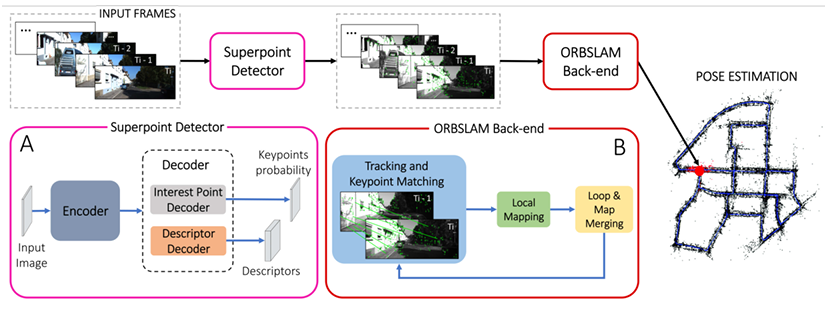
\includegraphics[width=0.8\textwidth]{images/superslam3.png}
    \caption{Integration of the Superpoint feature detector into the ORB-SLAM3 pipeline \cite{superslam3}.}
    \label{fig:superslam3_pipeline}
\end{figure}

\noindent\textbf{Advantages:} SUPERSLAM3 shows strong generalization across handheld, aerial, and automotive datasets without domain-specific weights, speeds up feature extraction relative to ORBSLAM3, and can outperform standard ORBSLAM3 in certain fast-motion indoor drone scenarios \cite{superpoint_slam3_2025,orbslam3}.

\noindent\textbf{Disadvantages:} It increases CPU memory use due to 256-element SuperPoint float descriptors, slows matching because it relies on $L_2$ distance rather than bit-wise ORB matching, and can suffer tracking drops or initialization failures in heavy motion blur or low-texture scenes \cite{superpoint_slam3_2025,superpoint,orbslam3}.

\subsubsection{SuperPoint SLAM3}
SuperPoint SLAM3 modifies the ORB-SLAM3 architecture by replacing handcrafted binary features with the \textbf{SuperPoint} network (DeTone et al., 2018) via the LibTorch C++ API. It utilizes 256-dimensional floating-point descriptors and implements Adaptive Non-Maximal Suppression (ANMS) to ensure uniform keypoint coverage across the image. The frontend matcher is rewritten to use Euclidean distance ($L_2$ norm) rather than the Hamming distance used for traditional binary features. \cite{orbslam3,superpoint_slam3_2025}

\begin{figure}[H]
    \centering
    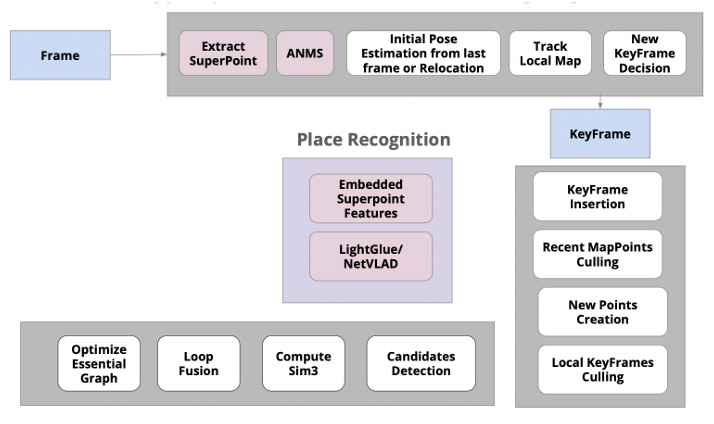
\includegraphics[width=0.8\textwidth]{images/superpoint_slam3.png}
    \caption{SuperPoint SLAM3 pipeline \cite{superpoint_slam3_2025}.}
    \label{fig:superpoint_slam3_pipeline}
\end{figure}


\begin{itemize}
    \item \textbf{Advantages:} This system reduces translational and rotational drift by providing more stable feature tracking. ANMS prevents keypoints from clustering in high-contrast areas, improving robustness in texture-sparse regions, while deep descriptors improve performance under illumination changes where standard ORB fails.
    \item \textbf{Disadvantages:} Floating-point descriptor matching is computationally heavier than binary operations, and storing 256-dimensional descriptors increases the memory footprint. Real-time operation typically requires a GPU, limiting deployment on ultra-low-power embedded devices.
\end{itemize}

\subsubsection{SELM SLAM3}
SELM-SLAM3 is designed for assistive navigation and is built using the ONNX Runtime C++ API to run \textbf{SuperPoint} (DeTone et al., 2018) and \textbf{LightGlue} (Lindenberger et al., 2023) natively without Python dependencies. It replaces standard projection-based tracking and Bag-of-Words matching with direct LightGlue inference, feeding current frames and local map points directly into the network to find correspondences. \cite{selm}

\begin{figure}[H]
    \centering
    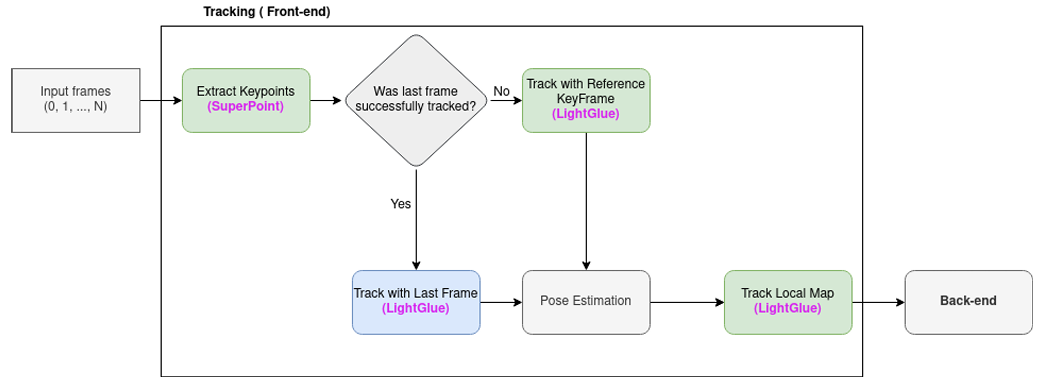
\includegraphics[width=0.8\textwidth]{images/selmslam.png}
    \caption{SELM-SLAM3 overview \cite{selm}.}
    \label{fig:selm_slam3_overview}
\end{figure}

\begin{itemize}
    \item \textbf{Advantages:} ONNX Runtime removes Python overhead, making the system easier to deploy and often faster than PyTorch-based hybrids. It offers strong robustness in low-texture scenes where heuristic matching fails and is optimized for erratic motion blur typical of wearable navigation aids.
    \item \textbf{Disadvantages:} Removing Bag-of-Words complicates loop closure and relocalization, requiring deep-learning replacements that increase compute. Despite using LightGlue, the end-to-end inference time for extraction and matching per frame remains higher than purely geometric approaches.
\end{itemize}

\subsubsection{Light-SLAM}
Light-SLAM addresses the lighting bottleneck of traditional methods by integrating a deep front-end using \textbf{SuperPoint} (DeTone et al., 2018) and \textbf{LightGlue} (Lindenberger et al., 2023) with a geometric backend. It incorporates an image enhancement module to restore gradient structures in low light and modifies the tracking thread to utilize LightGlue's adaptive depth mechanism, adjusting network inference complexity based on frame difficulty. \cite{lightslam,lightglue,superpoint}

\begin{figure}[H]
    \centering
    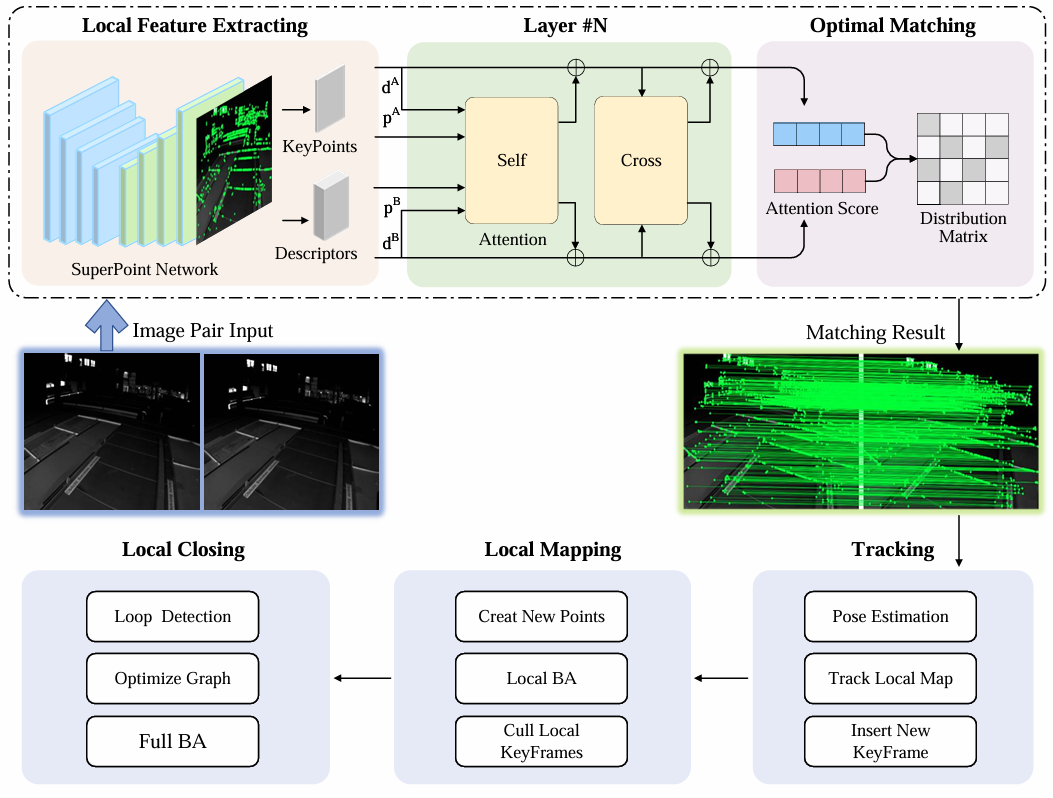
\includegraphics[width=0.8\textwidth]{images/lightslam.png}
    \caption{Light-SLAM architecture \cite{lightslam}.}
    \label{fig:lightslam_architecture}
\end{figure}


\begin{itemize}
    \item \textbf{Advantages:} Stable tracking in near-dark environments where traditional systems fail, with reduced compute on easy frames via early-stopping inference. Retains geometric accuracy of bundle adjustment while improving robustness under challenging illumination.
    \item \textbf{Disadvantages:} Still typically needs a CUDA-capable GPU, making it unsuitable for CPU-only platforms. Variable inference time can introduce jitter, which may affect control loops in autonomous robots.
\end{itemize}

\subsubsection{Deep-UAV SLAM}
Optimized for aerial robotics, Deep-UAV SLAM upgrades the ORB-SLAM3 front-end by integrating \textbf{SuperPoint} (DeTone et al., 2018) and \textbf{SuperGlue} (Sarlin et al., 2020) to handle bird's-eye views and rapid scale changes. A key innovation is retraining the Bag-of-Words vocabulary specifically for SuperPoint descriptors, enabling effective loop closure and relocalization. \cite{deepuav,superpoint,superglue}

\begin{figure}[H]
    \centering
    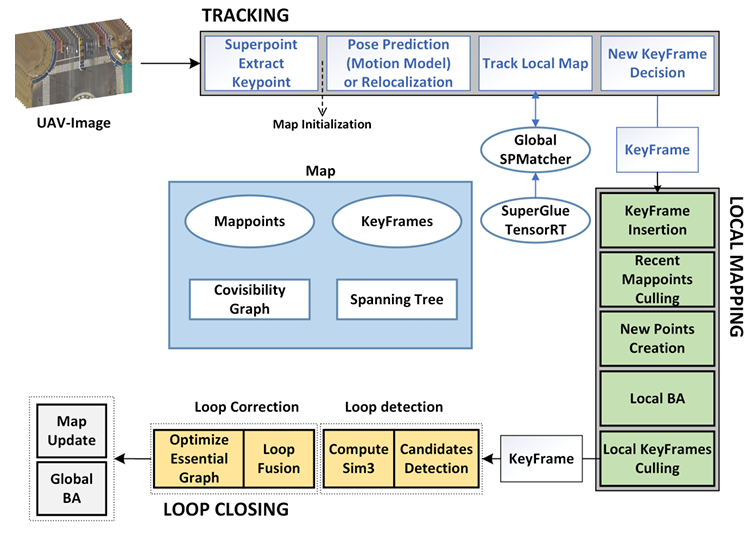
\includegraphics[width=0.8\textwidth]{images/deepuavslam.png}
    \caption{Deep-UAV SLAM pipeline \cite{deepuav}.}
    \label{fig:deepuavslam_pipeline}
\end{figure}

\begin{itemize}
    \item \textbf{Advantages:} Superior scale invariance for UAV altitude changes, improved robustness in dynamic outdoor aerial imagery, and a complete SLAM pipeline with functional relocalization and loop closure.
    \item \textbf{Disadvantages:} SuperGlue adds significant computational cost, typically requiring powerful edge AI hardware (e.g., Jetson-class). Building a Bag-of-Words vocabulary for continuous-space deep descriptors is complex and requires high-dimensional clustering.
\end{itemize}

\subsubsection{PCR-ORB}
PCR-ORB enhances the standard framework by integrating YOLOv8 for real-time semantic segmentation to identify and mask dynamic objects such as cars and people. It uses a CUDA-accelerated post-processing pipeline that refines the map by estimating the ground plane, removing sky artifacts, and enforcing temporal consistency on the point cloud. \cite{pcr}

\begin{figure}[H]
    \centering
    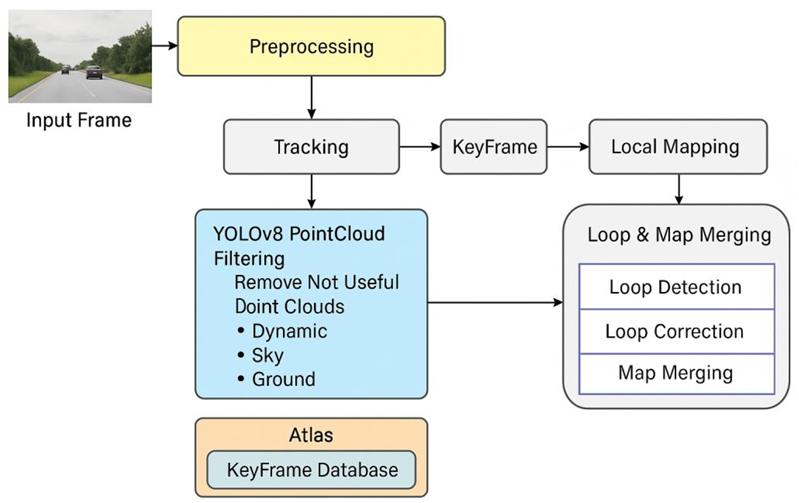
\includegraphics[width=0.8\textwidth]{images/pcrorb.png}
    \caption{PCR-ORB overview \cite{pcr}.}
    \label{fig:pcr_orb_overview}
\end{figure}

\begin{itemize}
    \item \textbf{Advantages:} Produces cleaner maps by reducing ghost trails from moving objects and removing sky artifacts. Improves robustness by avoiding feature lock-on to dynamic objects, adding semantic awareness to geometric SLAM.
    \item \textbf{Disadvantages:} Overhead can add latency in mostly static scenes with limited accuracy gains. Synchronizing heavy detection with the high-frequency tracking loop is challenging and can cause frame drops.
\end{itemize}

\noindent\textbf{Note:} The above method relies on SuperPoint for feature detection/description. \cite{superpoint}
\subsubsection{Summary}
\begin{table}[H]
\centering
\scriptsize % reduces font size
\caption{Comparison of Deep Learning-based VIO Algorithms}
\resizebox{\textwidth}{!}{%
\begin{tabular}{|p{1.5cm}|p{1.5cm}|p{1.5cm}|p{1.5cm}|p{4.5cm}|p{4.5cm}|}
\hline
\textbf{Algorithm} & \textbf{Deep Front-End} & \textbf{Deep Back-End} & \textbf{Primary Focus} & \textbf{Advantages} & \textbf{Disadvantages} \\
\hline

\hline
SUPER SLAM3 & Superpoint & Geometric SLAM + BoW (pre-trained) & Benchmark learned vs. handcrafted features &
\begin{itemize}[leftmargin=*, topsep=0pt, itemsep=0pt, parsep=0pt, partopsep=0pt]
  \item Generalizes across aerial, automotive, and handheld datasets with one pre-trained model.
  \item Faster keypoint/descriptor extraction than ORB.
\end{itemize} &
\begin{itemize}[leftmargin=*, topsep=0pt, itemsep=0pt, parsep=0pt, partopsep=0pt]
  \item Higher CPU memory from 256D float descriptors.
  \item Slower matching due to $L_2$ distance.
  \item Tracking degrades under heavy motion blur or low texture.
\end{itemize} \\
\hline

SuperPoint SLAM3 & SuperPoint & -- (geometric BA) & Robust feature tracking &
\begin{itemize}[leftmargin=*, topsep=0pt, itemsep=0pt, parsep=0pt, partopsep=0pt]
  \item Reduces translational/rotational drift via more stable learned features.
  \item Improved robustness under illumination changes; ANMS improves keypoint coverage in texture-sparse areas.
\end{itemize} &
\begin{itemize}[leftmargin=*, topsep=0pt, itemsep=0pt, parsep=0pt, partopsep=0pt]
  \item Heavier compute/memory than binary features due to floating-point descriptors and $L_2$ matching.
  \item Typically requires GPU for real-time performance on embedded platforms.
\end{itemize} \\
\hline

SELM-SLAM3 & SuperPoint + LightGlue & LightGlue correspondence inference & Robust matching (no BoW) &
\begin{itemize}[leftmargin=*, topsep=0pt, itemsep=0pt, parsep=0pt, partopsep=0pt]
  \item ONNX Runtime C++ deployment reduces Python overhead; often faster/easier to deploy than PyTorch hybrids.
  \item Strong robustness in low-texture scenes and under erratic motion blur.
\end{itemize} &
\begin{itemize}[leftmargin=*, topsep=0pt, itemsep=0pt, parsep=0pt, partopsep=0pt]
  \item Removing Bag-of-Words complicates loop closure/relocalization; deep replacements increase compute.
  \item End-to-end extraction+matching per frame can be slower than purely geometric approaches.
\end{itemize} \\
\hline

Light-SLAM & SuperPoint + LightGlue + image enhancement & Geometric backend & Low-light robustness &
\begin{itemize}[leftmargin=*, topsep=0pt, itemsep=0pt, parsep=0pt, partopsep=0pt]
  \item Stable tracking in near-dark environments; early-stopping inference reduces compute on easy frames.
  \item Retains geometric accuracy of bundle adjustment while improving robustness under challenging illumination.
\end{itemize} &
\begin{itemize}[leftmargin=*, topsep=0pt, itemsep=0pt, parsep=0pt, partopsep=0pt]
  \item Typically needs a CUDA-capable GPU; unsuitable for CPU-only platforms.
  \item Variable inference time may introduce jitter impacting real-time control loops.
\end{itemize} \\
\hline

Deep-UAV SLAM & SuperPoint + SuperGlue & Geometric SLAM + BoW (retrained) & Aerial robustness (scale/viewpoint) &
\begin{itemize}[leftmargin=*, topsep=0pt, itemsep=0pt, parsep=0pt, partopsep=0pt]
  \item Better scale invariance for UAV altitude changes; improved robustness for dynamic outdoor aerial imagery.
  \item Complete SLAM pipeline with functional relocalization and loop closure via retrained vocabulary.
\end{itemize} &
\begin{itemize}[leftmargin=*, topsep=0pt, itemsep=0pt, parsep=0pt, partopsep=0pt]
  \item SuperGlue adds significant computational cost (often needs Jetson-class hardware).
  \item Building BoW for high-dimensional deep descriptors is complex and expensive.
\end{itemize} \\
\hline

PCR-ORB & YOLOv8 (semantic masking) & Geometric SLAM + point-cloud refinement & Dynamic-object handling / clean maps &
\begin{itemize}[leftmargin=*, topsep=0pt, itemsep=0pt, parsep=0pt, partopsep=0pt]
  \item Cleaner maps by masking dynamic objects and removing sky/ground artifacts via post-processing.
  \item More robust tracking by avoiding features on moving objects (adds semantic awareness).
\end{itemize} &
\begin{itemize}[leftmargin=*, topsep=0pt, itemsep=0pt, parsep=0pt, partopsep=0pt]
  \item Added latency/overhead in mostly static scenes with limited gains.
  \item Synchronizing heavy detection with high-rate tracking is challenging; can cause frame drops.
\end{itemize} \\
\hline
\end{tabular}}
\label{tab:DL_VINS_comparison}
\end{table}




\section{Experimental Evaluations}
This section summarizes the evaluation setup, platforms, and observed performance of representative VIO/VSLAM systems under comparable flight conditions. The focus is on localization stability, drift characteristics, and qualitative trajectory consistency in GPS-denied scenarios. Where applicable, both quantitative metrics (e.g., tracking quality, ATE, offsets) and qualitative observations (e.g., path coherence, landmark distribution) are reported.
\subsection{Evaluation Platforms}
\subsubsection{ModalAI Starling 2 Max}
The Starling 2 Max by ModalAI integrates the VOXL 2 companion computer, integrated stereo tracking cameras for visual--inertial odometry, and a forward-facing RGB camera for vision-based perception. It is designed for autonomous navigation and AI research in GPS-denied environments.

\subsubsection{Custom UAV Platform}
Our custom UAV platform integrates an NVIDIA Jetson Orin NX 16GB companion computer and an Orbbec Gemini 2L RGB-D camera with a built-in IMU. The platform is designed for high-performance visual--inertial navigation and autonomous flight.

\subsection{Evaluation Results}
\noindent\textbf{Test Conditions:} Evaluations were conducted under good lighting with textured surfaces to ensure sufficient visual features. Each system was assessed for tracking continuity, drift behavior, and consistency between IMU and VIO estimates.

\subsubsection{OpenVINS}
OpenVINS demonstrated stable localization during the test run, achieving a tracking quality of 96\%. The IMU-to-VIO translation offsets remained small (\(\leq 0.09~\text{m}\)), and attitude angles stayed within \(\pm 1.4^{\circ}\), indicating minimal drift. The drone path visualization confirms a tight, controlled trajectory with well-distributed feature landmarks, consistent with reliable odometry under good lighting and textured surfaces.

\subsubsection{qVIO}
qVIO completed the test run but showed notably lower tracking quality at 75\%. The IMU-to-VIO translation offsets were larger (up to \(0.55~\text{m}\)), and attitude angles diverged more significantly, with yaw reaching \(-12.1^{\circ}\). The drone path visualization reflects this, with visible drift and looser path coherence compared to OpenVINS, suggesting higher susceptibility to accumulated estimation error under the same flight conditions.

\subsubsection{PyCuVSLAM}
PyCuVSLAM achieved stable tracking with moderate drift. Its GPU-accelerated pipeline maintained consistent pose estimates and supported loop-closure behavior, but trajectory smoothness was dependent on available GPU resources and system load. Overall performance was stronger than pure VIO baselines but less consistent than ORB-SLAM3 under identical conditions.

\subsubsection{ORB-SLAM3}
ORB-SLAM3 produced the most globally consistent trajectory in the tests. Loop closure and map reuse reduced long-term drift, yielding a tight path with minimal accumulated error. Tracking stability was strong, though the system required higher compute and careful initialization to avoid early-stage failures.

\subsection{Discussion}
Overall, OpenVINS exhibited stronger short-term stability and tighter trajectory consistency under the tested conditions, while qVIO showed larger accumulated errors and reduced tracking quality. These outcomes align with the expected behavior of pure VIO systems that lack loop-closure mechanisms and are therefore more vulnerable to long-term drift.

\subsection{Summary}
\begin{table}[H]
\centering
\caption{Comparison of VIO/VSLAM Frameworks}
\label{tab:vio_vslam_summary}
\begin{tabular}{|p{2.6cm}|p{3.6cm}|p{3.4cm}|p{3.8cm}|}
\hline
\textbf{Framework} & \textbf{Absolute Trajectory Error (ATE)} & \textbf{Long-Term Drift} & \textbf{Loop Closure / Map Reuse} \\
\hline
ORB-SLAM3 & 0.01--0.03 m & Eliminated & Yes (Global Map) \\
\hline
PyCuVSLAM & 0.1 m & Moderate & Yes \\
\hline
OpenVINS & 0.05 m & Accumulates over time & No (Pure VIO) \\
\hline
qVIO & 0.5 m & Accumulates over time & No (Pure VIO) \\
\hline
\end{tabular}
\end{table}
\section{Methodology}
\sloppy

\subsection{Proposed Solution}
To address the navigation challenges in GPS-restricted environments, the proposed solution implements a tightly-coupled, real-time Visual-Inertial Navigation System (VINS) utilizing the ORB-SLAM3 framework in RGBD-Inertial mode. This architecture leverages an NVIDIA Jetson Orin NX companion computer for high-performance processing and an Orbbec Gemini 2L camera to provide synchronized RGB, depth, and 200Hz IMU data. By utilizing aligned depth maps, the system establishes an absolute metric scale from the initial frame, effectively eliminating the scale ambiguity and initialization delays common in monocular systems. The software pipeline, orchestrated via ROS 2 Humble, integrates a custom VIO Bridge to manage frame transformations and coordinate alignment, ensuring the SLAM-derived poses are accurately fused into the Pixhawk 6X Pro flight controller's EKF2 estimator through the MAVROS bridge for stable, closed-loop autonomous flight

\subsection{System Architecture}
The VIO system follows a modular pipeline architecture consisting of four ROS 2 nodes spread across three custom packages, orchestrated to provide seamless state estimation. The pipeline processes sensor data through a well-defined chain: raw camera and IMU data $\rightarrow$ visual SLAM $\rightarrow$ frame transformation and heading correction $\rightarrow$ flight controller integration \cite{ros2_humble,mavros_wiki,px4_user_guide}.

\begin{figure}[H]
    \centering
    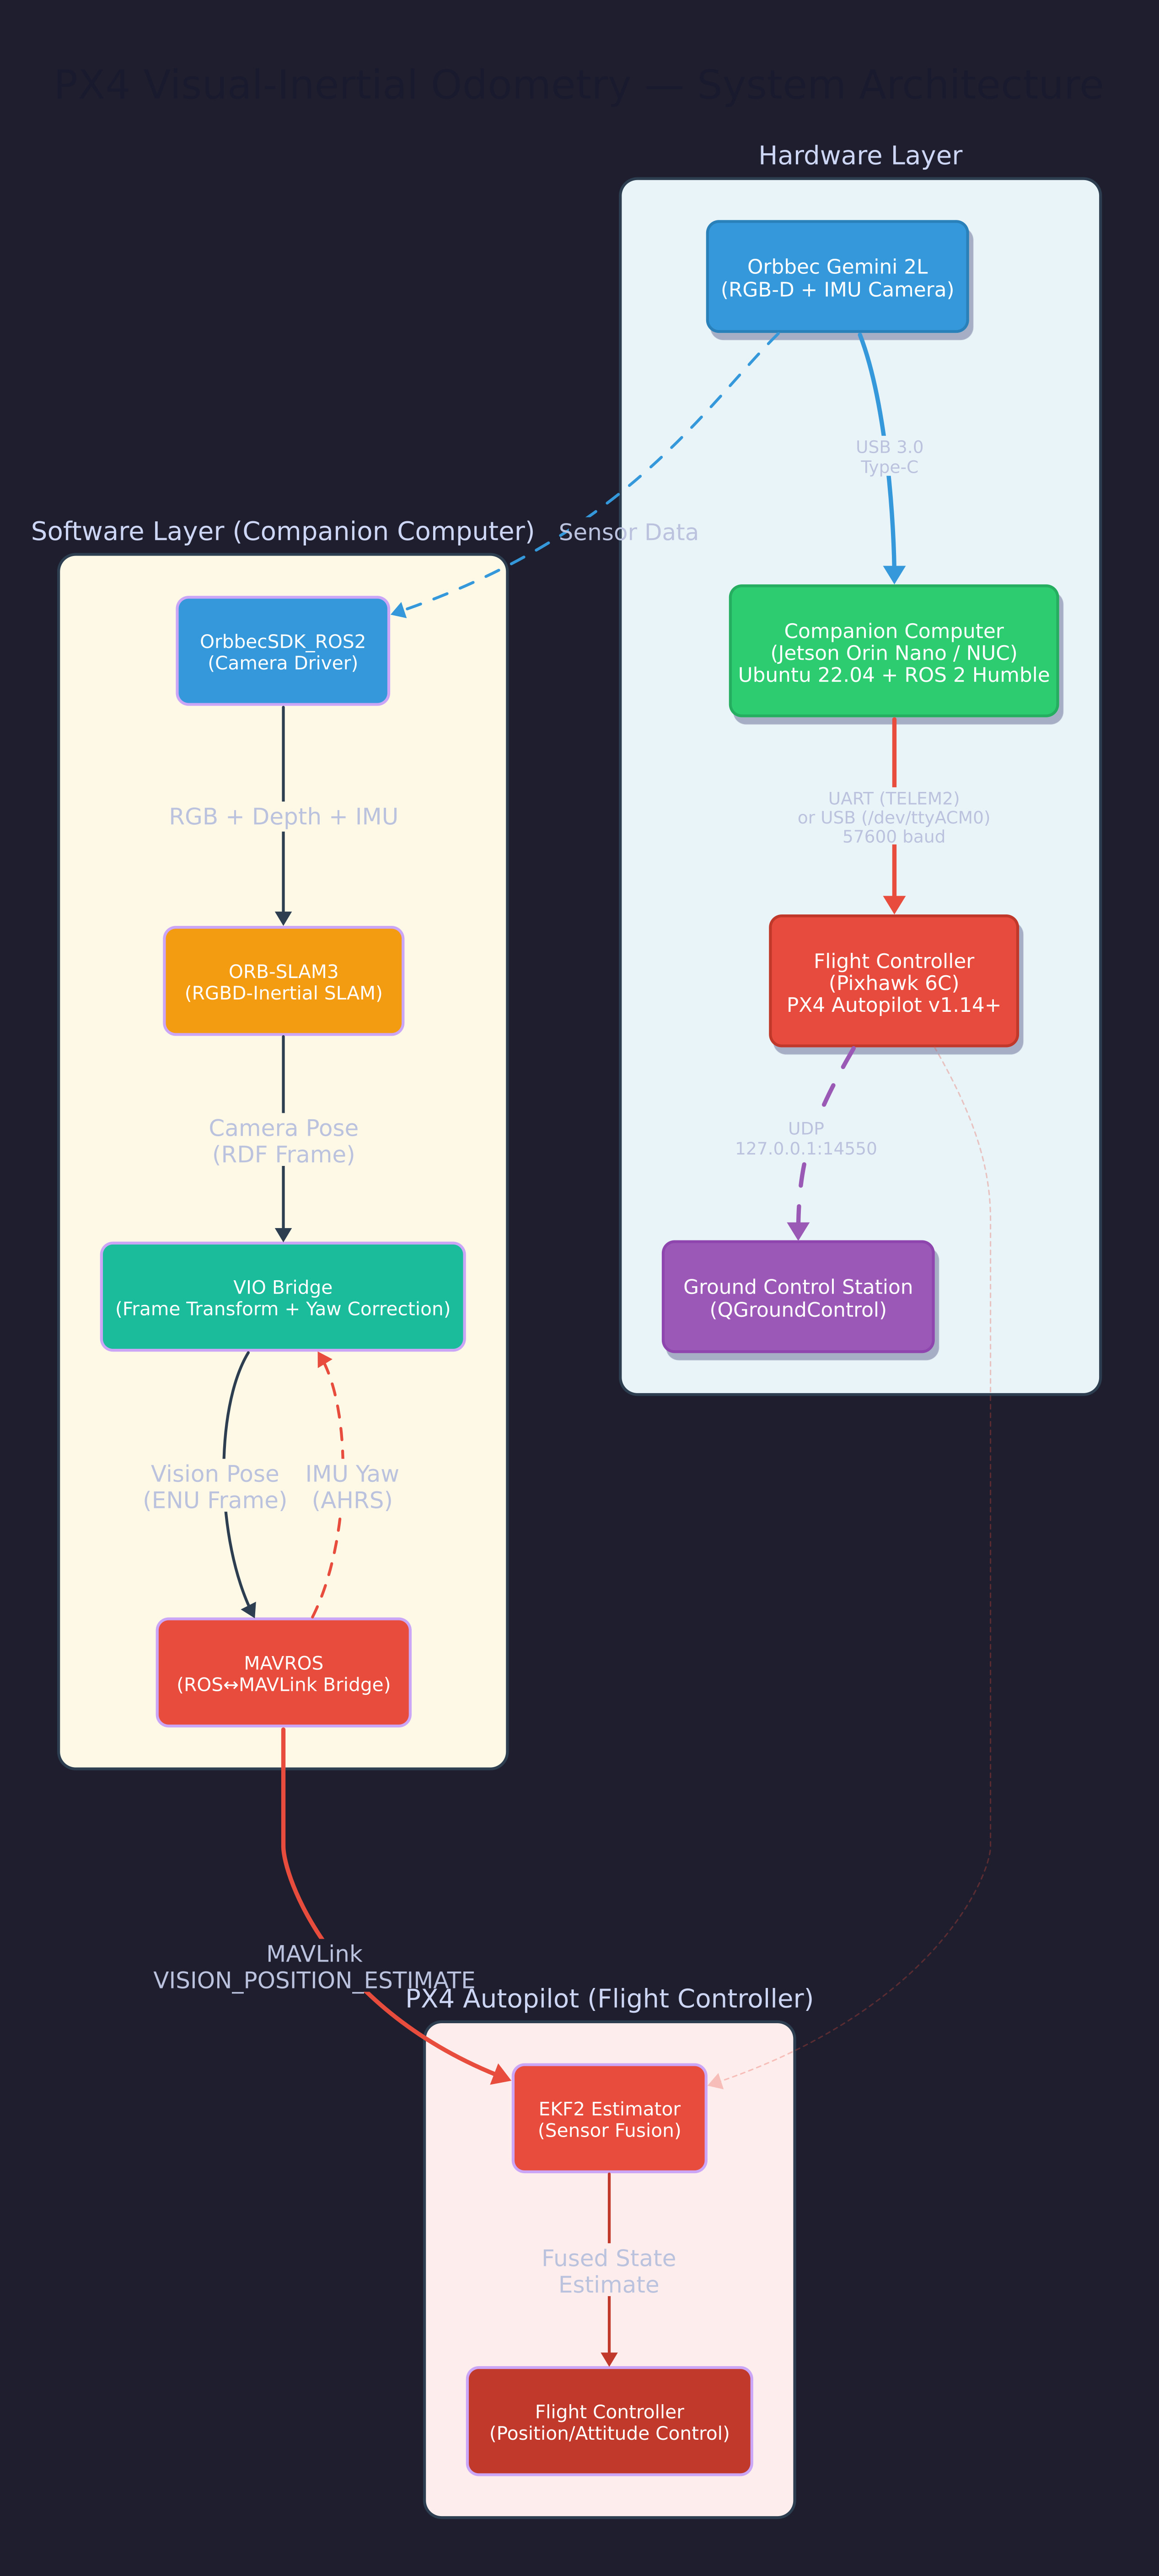
\includegraphics[width=\linewidth,height=0.75\textheight,keepaspectratio]{images/01_system_architecture.jpg}
    \caption{System architecture overview of the ROS~2-based VIO/navigation stack.}
    \label{fig:system_architecture}
\end{figure}

The architecture is deliberately focused on the core VIO pipeline, prioritizing robustness and low latency over feature complexity. Each node has a single, well-defined responsibility, making the system easier to debug, maintain, and validate in real flight conditions.


\begin{table}[H]
\centering
\scriptsize % reduces font size
\caption{ROS Nodes}
\resizebox{\textwidth}{!}{%
\begin{tabular}{|p{2.8cm}|p{2.6cm}|p{6.6cm}|p{4.2cm}|}
\hline \textbf{Node} & \textbf{Package} & \textbf{Role} & \textbf{Key Output} \\

\hline Orbbec Camera Node & OrbbecSDK\_ROS2 & Publishes synchronized RGB, Depth, and IMU data from the Gemini 2L camera \cite{orbbec_ros2_sdk} & RGB images (30Hz), Depth maps (30Hz), IMU (200Hz) \\

\hline ORB-SLAM3 Node & orbslam3\_ros2 & Performs RGBD-Inertial SLAM --- extracts features, fuses IMU, and estimates camera pose & 6-DOF Camera Pose in gravity-aligned world \\

\hline VIO Bridge Node & vio\_bridge & Transforms SLAM pose (RDF$\rightarrow$ENU), applies yaw correction, monitors drift, detects resets & Corrected Body Pose in ENU frame \\

\hline MAVROS Node & mavros & Bridges ROS 2 to PX4 via MAVLink --- converts ENU$\rightarrow$NED and sends vision pose estimates & VISION\_POSITION\_ESTIMATE MAVLink message \\

\hline \end{tabular}}
\label{tab:ros_nodes}
\end{table}

\subsection{Hardware Platform}
The system is built on the Holybro Jetson Pack — an integrated carrier board solution that combines the NVIDIA Jetson Orin NX 16GB module with the Holybro Pixhawk 6X Pro flight controller \cite{holybro_jetson_pack,jetson_orin_nx_datasheet,pixhawk6x_datasheet}. This provides a compact, flight-ready package with direct inter-processor communication, eliminating the need for external wiring between the companion computer and the autopilot \cite{holybro_jetson_pack}.

\begin{table}[H]
\centering
\scriptsize
\caption{Hardware Components}
\setlength{\tabcolsep}{3pt}% tighten columns (helps keep height down)
\renewcommand{\arraystretch}{0.9}% tighten row spacing (helps keep height down)
\resizebox{\textwidth}{!}{%
\begin{tabular}{|p{3.0cm}|p{3.2cm}|p{7.3cm}|p{7.3cm}|}
\hline
\textbf{Component} & \textbf{Model} & \textbf{Specification} & \textbf{Reason for Choosing} \\

\hline
Companion Computer & NVIDIA Jetson Orin NX 16GB (Holybro Jetson Pack) &
Ubuntu 22.04, ROS 2 Humble, 16GB LPDDR5 RAM, 8-core ARM Cortex-A78AE, 1024-core Ampere GPU, 100 TOPS AI\cite{jetson_orin_nx_datasheet} &
Provides high-performance onboard GPU acceleration required for real-time SLAM, visual processing, and autonomous navigation \\

\hline
RGB-D Camera & Orbbec Gemini 2L &
1280$\times$800 RGB @ 30fps, aligned depth @ 30fps, on-board IMU @ 200Hz, 100\,mm stereo baseline\cite{orbbec_gemini2l_datasheet} &
Provides synchronized RGB, depth, and inertial data required for accurate visual-inertial SLAM \\

\hline
Flight Controller & Holybro Pixhawk 6X Pro (PX4 v1.14+) &
STM32H7 processor, triple redundant IMU, EKF2 estimator, MAVLink telemetry\cite{pixhawk6x_datasheet} &
Provides reliable flight control and supports external vision-based position estimation for GPS-denied navigation \\

\hline
Battery & CNHL LiPo 4S 5200mAh &
14.8\,V nominal voltage, 5200mAh capacity, high discharge rate LiPo battery\cite{cnhl_5200mah_datasheet} &
Provides sufficient power capacity and stable voltage supply for flight controller, companion computer, and onboard sensors \\

\hline
Drone Frame & S500 Quadcopter Frame &
500\,mm wheelbase, lightweight composite frame, supports quad-motor configuration\cite{s500_frame_specs} &
Provides stable structure with sufficient payload capacity and mounting space for onboard computing and sensing hardware \\

\hline
Motors (×4) & 2212 920KV Brushless Motors &
920KV rating, supports 2--4S LiPo, max current $\sim$18A, thrust $\sim$500g per motor\cite{motor_2212_920kv} &
Provides sufficient thrust-to-weight ratio and efficient performance for stable autonomous flight \\

\hline
Propellers (×4) & 9450 Propellers &
9.4-inch diameter, 5.0-inch pitch, compatible with 2212 motors\cite{propeller_9450} &
Provides efficient thrust generation and aerodynamic stability for quadcopter operation \\

\hline
Electronic Speed Controller (×4) & SimonK 30A ESC &
30A continuous current, supports 2--4S LiPo, fast response firmware\cite{motor_2212_920kv} &
Provides reliable and precise motor speed control required for stable flight and attitude control \\

\hline
RF Receiver & RadioMaster ER6 Receiver &
2.4\,GHz ExpressLRS receiver, 6 channels, low latency, long range\cite{radiomaster} &
Provides reliable manual control capability for testing, safety override, and system calibration \\

\hline
WiFi Telemetry Module & CUAV PW-Link Module &
2.4\,GHz WiFi telemetry, MAVLink support, UART interface, low latency communication\cite{cuav_pwlink_datasheet} &
Enables wireless telemetry communication between UAV and ground station for monitoring and control \\
\hline

\end{tabular}}
\label{tab:hardware_components}
\end{table}


The Holybro Jetson Pack carrier board provides a direct UART connection between the Jetson Orin NX and the Pixhawk 6X Pro, removing the need for USB adapters or external serial converters. The 16GB of LPDDR5 RAM ensures headroom for ORB-SLAM3's memory-intensive map management alongside camera processing and ROS 2 overhead.

\subsection{Software Stack}
The software environment and key dependencies are as follows:

\begin{table}[H]
\centering
\scriptsize
\caption{Software Stack}
\resizebox{\textwidth}{!}{%
\begin{tabular}{|p{3.2cm}|p{4.2cm}|p{9.8cm}|}
\hline \textbf{Software} & \textbf{Version} & \textbf{Purpose} \\

\hline Ubuntu & 22.04 LTS (Jammy) & Base operating system (JetPack 6.x compatible) \cite{ubuntu_2204} \\

\hline ROS 2 & Humble Hawksbill & Middleware framework for inter-node communication \cite{ros2_humble} \\

\hline OrbbecSDK\_ROS2 & Latest & Camera driver with synchronized IMU output \cite{orbbec_ros2_sdk} \\

\hline MAVROS & ROS 2 Humble release & MAVLink bridge to PX4 flight controller \cite{mavros_wiki} \\

\hline PX4 Autopilot & v1.14+ & Flight controller firmware with EKF2 vision fusion \cite{px4_user_guide} \\

\hline CUDA Toolkit & 11.x / 12.x & Enables GPU acceleration for SLAM, deep learning, and image processing \\

\hline OpenCV & 4.x (with CUDA) & Image processing and feature extraction with GPU acceleration \\

\hline QGroundControl & v4.x & Ground control station for UAV configuration, telemetry, and mission testing \\

\hline
\end{tabular}}
\label{tab:software_stack}
\end{table}

\subsection{Sensor Data Aquisition}
The Orbbec Gemini 2L camera provides all perceptual data for the SLAM system through three synchronized data streams \cite{orbbec_gemini2l_datasheet}. The camera's on-board IMU eliminates the need for an external inertial sensor, simplifying the hardware setup and reducing extrinsic calibration complexity \cite{orbbec_gemini2l_datasheet}.

\begin{figure}[H]
    \centering
    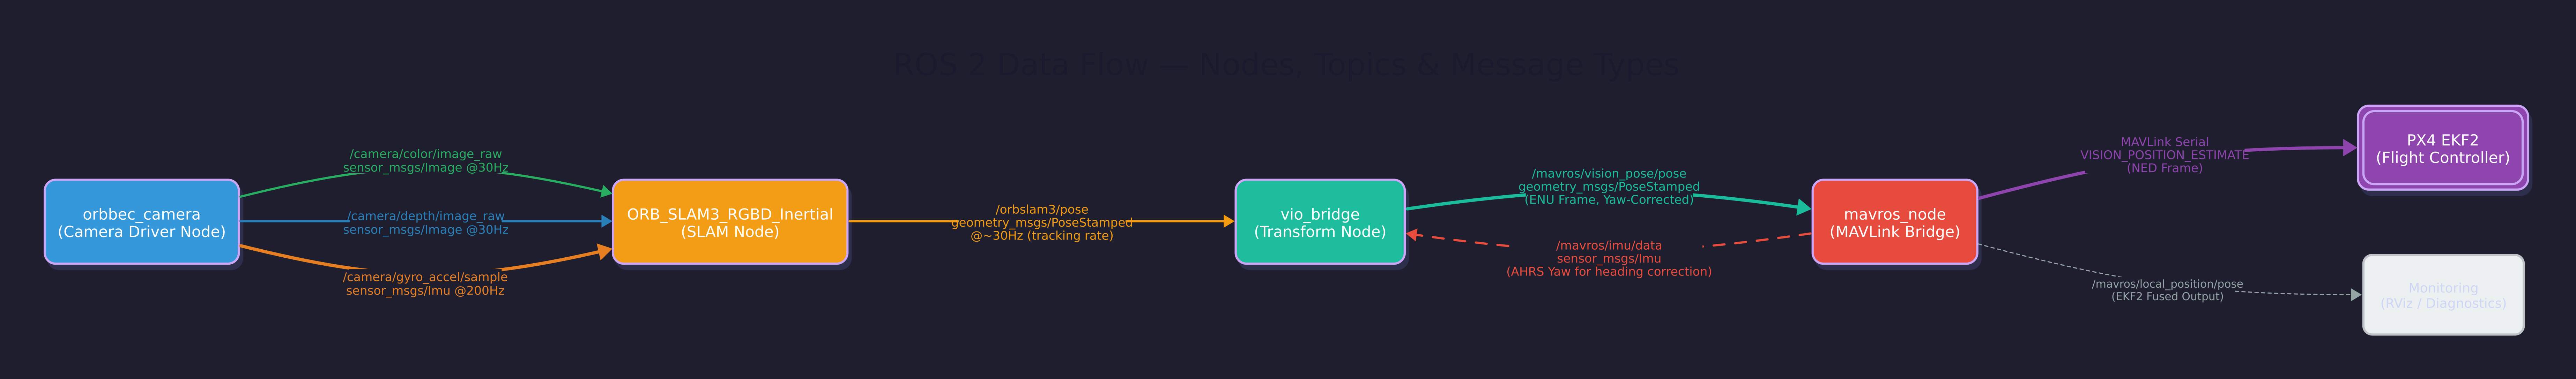
\includegraphics[width=\linewidth,height=0.75\textheight,keepaspectratio]{images/02_ros2_dataflow.jpg}
    \caption{ROS2 Data Flow.}
    \label{fig:data_flow}
\end{figure}

\begin{table}[H]
\centering
\scriptsize % reduces font size
\caption{ROS 2 Sensor Topics}
\resizebox{\textwidth}{!}{%
\begin{tabular}{|p{4.2cm}|p{3.2cm}|p{1.4cm}|p{2.0cm}|p{7.0cm}|}
\hline \textbf{ROS 2 Topic} & \textbf{Message Type} & \textbf{Rate} & \textbf{Resolution} & \textbf{Purpose} \\

\hline /camera/color/image\_raw & sensor\_msgs/Image & 30 Hz & 1280$\times$800 & RGB frames for ORB feature extraction and visual tracking \\

\hline /camera/depth/image\_raw & sensor\_msgs/Image & 30 Hz & 1280$\times$800 & Aligned depth maps for 3D scale estimation (resolves monocular ambiguity) \\

\hline /camera/gyro\_accel/sample & sensor\_msgs/Imu & 200 Hz & N/A & Fused accelerometer + gyroscope for IMU preintegration in ORB-SLAM3 \\

\hline \end{tabular}}
\label{tab:ros2_sensor_topics}
\end{table}

The synchronized accel/gyro output is critical — the camera driver merges both IMU streams into a single topic at 200 Hz, which ORB-SLAM3 buffers and preintegrates between image frames.

\subsection{Visual Inertial SLAM (ORB-SLAM3)}
ORB-SLAM3 operates in RGBD-Inertial mode, tightly coupling visual feature observations with IMU preintegration constraints. This mode was chosen over pure visual or monocular-inertial alternatives because the depth sensor provides absolute metric scale from the first frame, eliminating the scale ambiguity and delayed initialization problems of monocular approaches.

\begin{figure}[!ht]
    \centering
    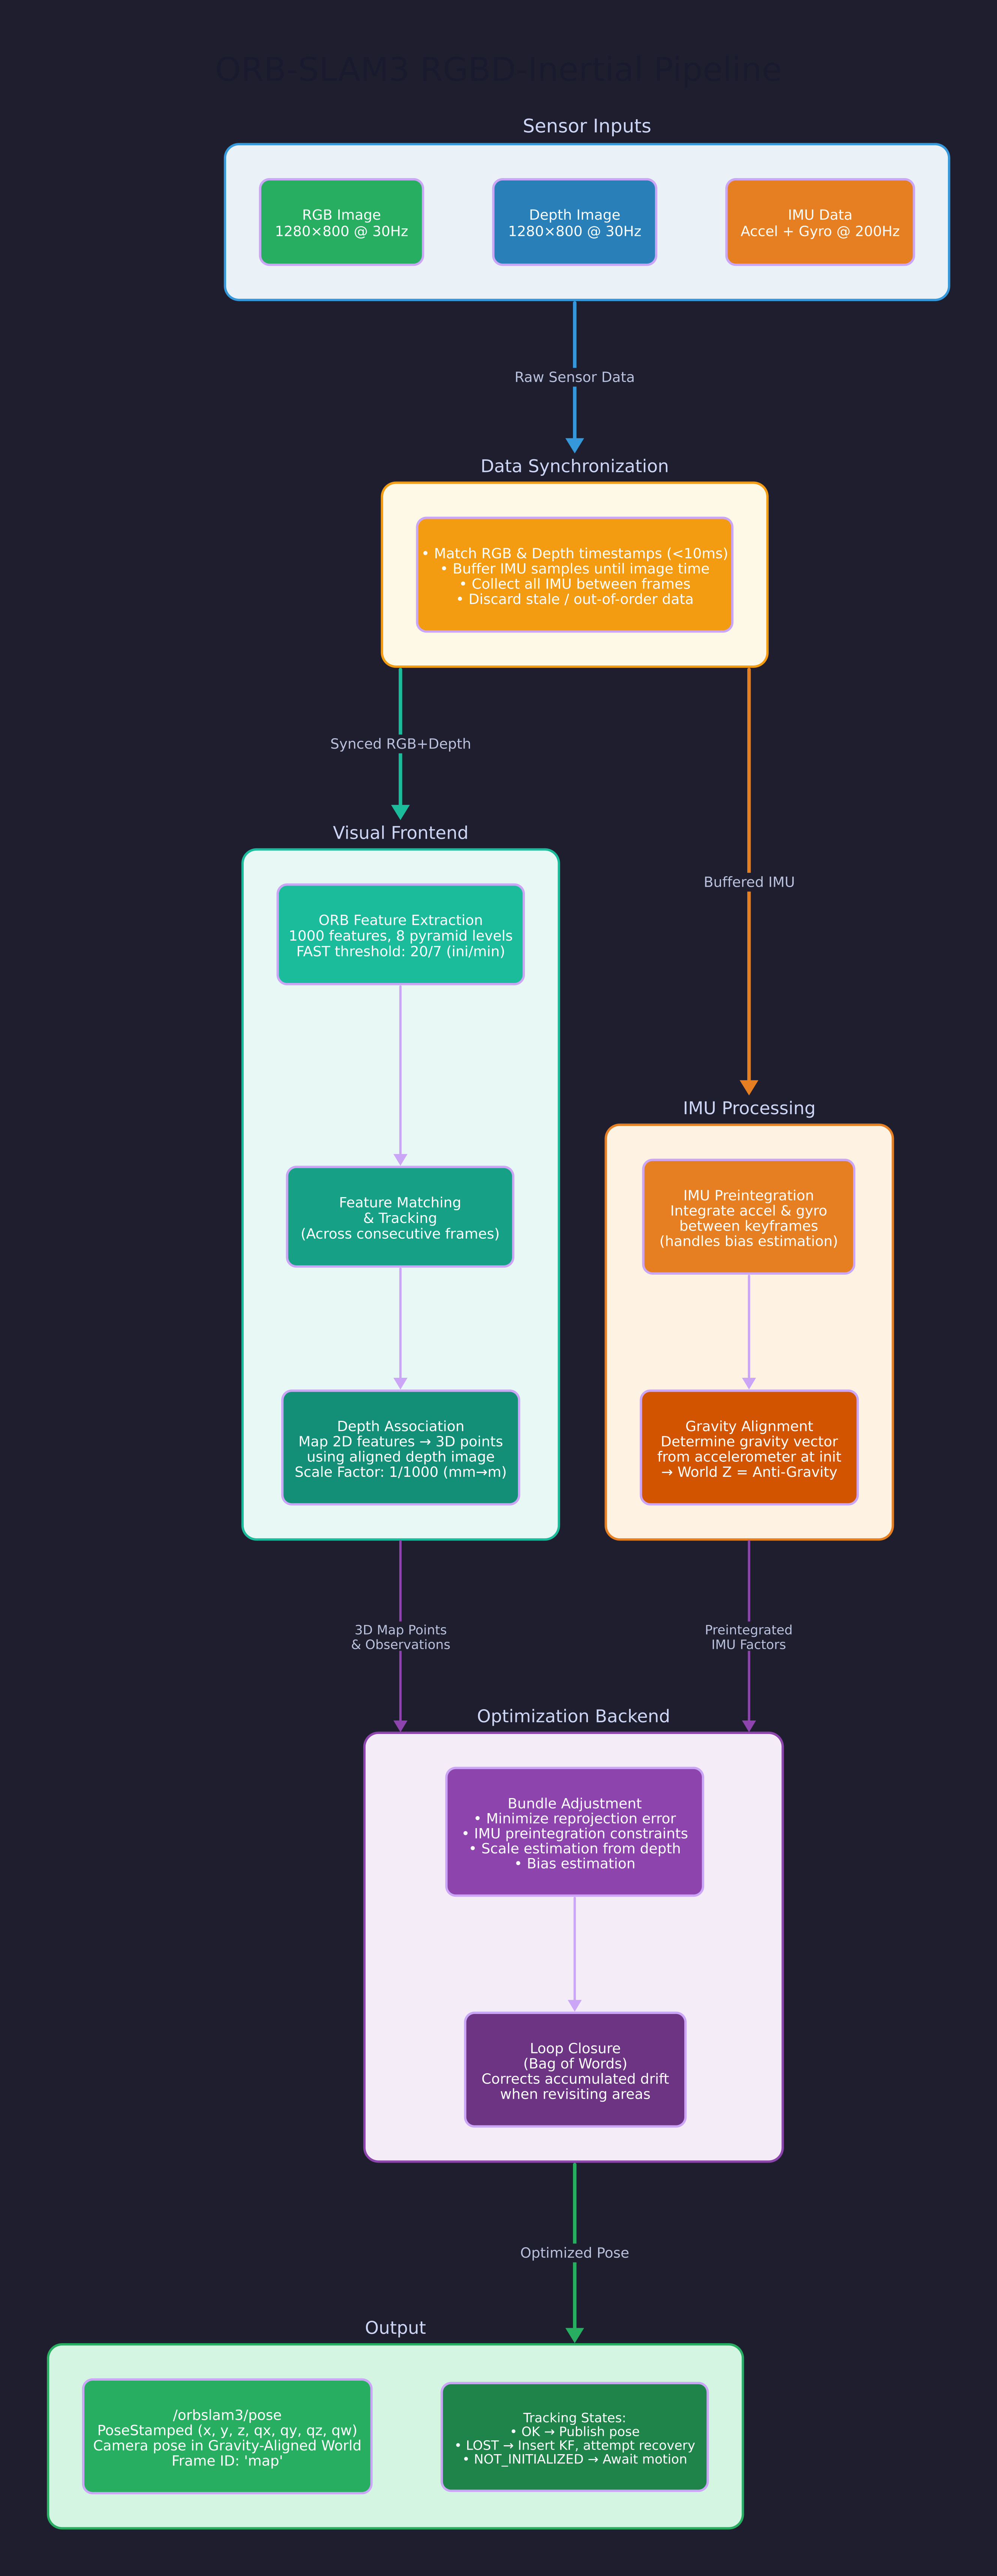
\includegraphics[width=\linewidth,height=0.75\textheight,keepaspectratio]{images/06_orbslam3_pipeline.jpg}
    \caption{ORB-SLAM3 RGBD-Inertial Processing Pipeline}
    \label{fig:data_flow}
\end{figure}

\subsubsection{Processing Pipeline}
\begin{enumerate}
    \item \textbf{Data Synchronization:} RGB and depth frames are matched within 10\,ms tolerance. IMU measurements are buffered and associated with the nearest image timestamp.
    \item \textbf{Feature Extraction:} ORB features are extracted from the RGB image --- 1000 features across 8 pyramid levels (scale factor 1.2), with adaptive FAST thresholds (initial: 20, minimum: 7).
    \item \textbf{Depth Association:} Each detected 2D feature is associated with its depth value from the aligned depth map, creating 3D landmarks with known metric scale.
    \item \textbf{IMU Preintegration:} Accelerometer and gyroscope measurements between consecutive frames are preintegrated to predict inter-frame motion, providing short-term odometry even when visual tracking is poor.
    \item \textbf{Tracking \& Optimization:} The system performs local Bundle Adjustment, jointly optimizing camera poses, 3D landmarks, and IMU biases to minimize reprojection error and inertial residuals.
    \item \textbf{Gravity Alignment:} During initialization, the IMU accelerometers determine the gravity vector. The world frame is rotated so its Z-axis aligns with vertical (against gravity), producing a horizon-level reference.
    \item \textbf{Loop Closure:} Bag-of-Words place recognition detects revisited locations and triggers a global pose-graph optimization to correct accumulated drift.
\end{enumerate}

\subsubsection{Key Configuration Parameters}
The ORB-SLAM3 configuration was optimized specifically for the Orbbec Gemini 2L camera's characteristics (file: \texttt{Orbbec\_Gemini2L\_Optimized.yaml}):

\begin{table}[H]
\centering
\scriptsize % reduces font size
\caption{ORB-SLAM3 Configuration Parameters}
\resizebox{\textwidth}{!}{%
\begin{tabular}{|p{4.2cm}|p{4.2cm}|p{7.4cm}|}
\hline \textbf{Parameter} & \textbf{Value} & \textbf{Justification} \\

\hline Camera1.fx / fy & 606.96 / 607.11 & Focal lengths from device intrinsic calibration \\

\hline Camera1.cx / cy & 637.73 / 392.85 & Principal point from device calibration \\

\hline Distortion ($k_1$--$k_3$, $p_1$--$p_2$) & -0.897, 0.252, 0.000, -0.001, 0.037 & Plumb-bob distortion model correcting barrel distortion \\

\hline RGBD.DepthMapFactor & 1000.0 & Converts depth from millimeters (sensor native) to meters \\

\hline Stereo.b (baseline) & 0.10 m & 100\,mm stereo baseline of the Gemini 2L \\

\hline IMU.NoiseGyro / NoiseAcc & 2.0e-2 / 2.0e-1 & Tuned higher than datasheet --- improves stability when stationary \\

\hline IMU.Frequency & 200 Hz & Matches camera IMU output rate \\

\hline IMU.fastInit & 0 (disabled) & Allows more robust initialization; avoids premature lock with noisy IMU \\

\hline \end{tabular}}
\label{tab:orbslam3_config_params}
\end{table}

\subsection{VIO Bridge - Frame Transformation \& Yaw Correction}
The VIO Bridge is a custom ROS 2 C++ node (\texttt{vio\_bridge\_node.cpp}) that serves as the critical middleware between the SLAM system and the flight controller. It performs three essential functions: coordinate frame rotation, heading alignment, and health monitoring.

\begin{figure}[!ht]
    \centering
    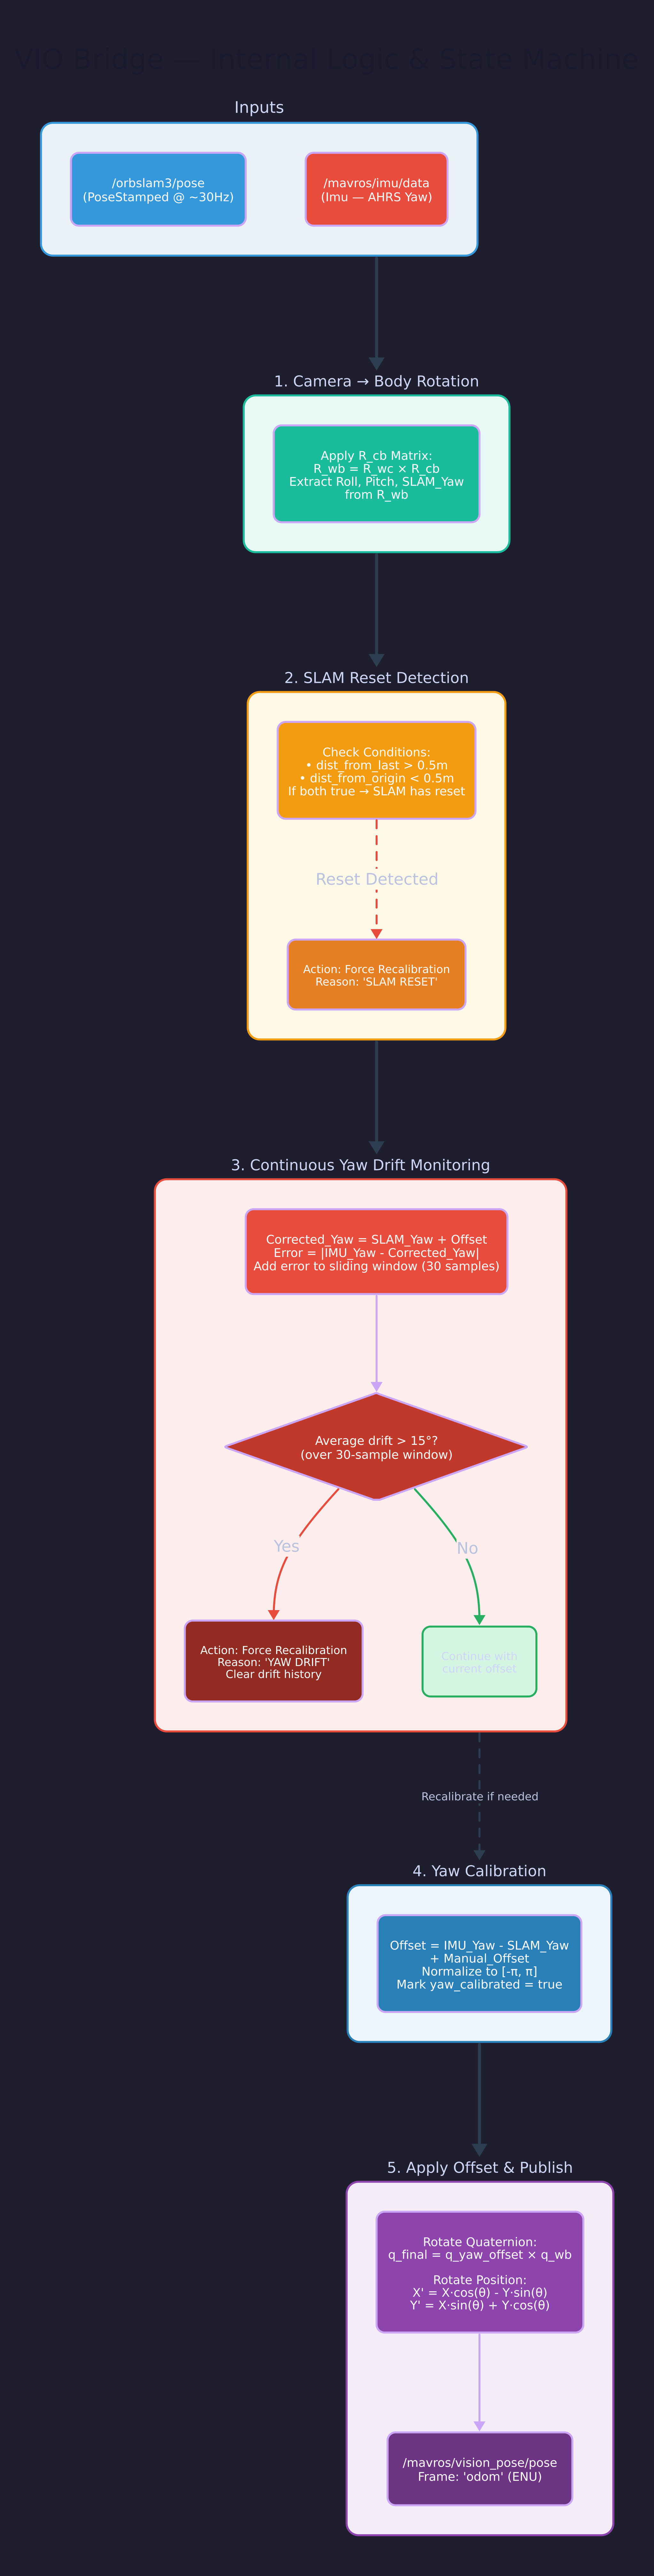
\includegraphics[width=\linewidth,height=0.75\textheight,keepaspectratio]{images/05_vio_bridge_logic.jpg}
    \caption{VIO Bridge Internal Logic }
    \label{fig:data_flow}
\end{figure}

\subsubsection{Camera-to-Body Frame Rotation}
\noindent ORB-SLAM3 outputs the camera pose in an Optical Frame convention (Right-Down-Forward, RDF). The flight controller expects poses in a Body Frame convention (Forward-Left-Up, FLU) aligned with the East-North-Up (ENU) world. The bridge applies a static rotation matrix $R_{cb}$:
\[
R_{cb} =
\begin{pmatrix}
0 & -1 & 0 \\
0 & 0 & -1 \\
1 & 0 & 0
\end{pmatrix}
\]
This maps:
\begin{itemize}
    \item Camera $Z$ (Forward) $\rightarrow$ Body $X$ (Forward)
    \item Camera $X$ (Right) $\rightarrow$ Body $-Y$ (Right, since Body $Y$ is Left)
    \item Camera $Y$ (Down) $\rightarrow$ Body $-Z$ (Down, since Body $Z$ is Up)
\end{itemize}
The full transformation is:
\[
T_{wb} = T_{wc} \times T_{cb},
\]
converting the World-to-Camera pose into a World-to-Body pose.

\subsubsection{Yaw Heading Correction}
ORB-SLAM3 initializes with an arbitrary yaw (Yaw = 0 at startup), which does not correspond to any real-world heading. PX4 requires that the vision pose heading is consistent with its internal heading estimate (derived from the magnetometer via the AHRS). The bridge implements the following yaw alignment algorithm:
\begin{enumerate}
    \item \textbf{Subscribe:} to \texttt{/mavros/imu/data} to obtain the current AHRS yaw from PX4.
    \item \textbf{Calculate Offset:} $\textit{yaw\_offset} = \textit{IMU\_Yaw} - \textit{SLAM\_Yaw}$ (at the first valid pose or after recalibration).
    \item \textbf{Apply Correction:} Rotate both the orientation quaternion and the position vector by the yaw offset. This ensures the entire trajectory is rotated to align with the real heading.
    \item \textbf{Position Rotation:} $x_{\text{final}} = x\cdot\cos(\textit{offset}) - y\cdot\sin(\textit{offset});\; y_{\text{final}} = x\cdot\sin(\textit{offset}) + y\cdot\cos(\textit{offset})$. This accounts for the fact that the SLAM coordinate axes must also be rotated, not just the heading.
\end{enumerate}

\subsubsection{Continuous Drift Monitoring}
SLAM heading can drift over time relative to the magnetometer. The bridge implements a sliding-window drift detector:
\begin{itemize}
    \item \textbf{Window Size:} 30 samples --- the bridge tracks the absolute yaw error between the corrected SLAM yaw and the IMU yaw over the last 30 SLAM poses.
    \item \textbf{Threshold:} $15^\circ$ --- if the average drift across the window exceeds 15 degrees, the bridge triggers an automatic recalibration (re-computes the yaw offset).
    \item \textbf{Hysteresis:} After recalibration, the drift history is cleared to prevent oscillating corrections.
\end{itemize}

\subsubsection{SLAM Reset Detection}
If ORB-SLAM3 loses tracking and re-initializes, the position jumps back to the origin. This would cause a dangerous discontinuity for PX4. The bridge detects this condition by monitoring the position: if the distance from the previous position exceeds 0.5\,m \textbf{and} the distance from the origin is less than 0.5\,m, a ``SLAM Reset'' is declared and the yaw offset is immediately recalibrated.

\subsubsection{Diagnostics}
The bridge runs a diagnostic timer every 5 seconds that logs: current publish rate (Hz), average yaw drift (degrees), SLAM reset count, and drift recalibration count. This provides real-time health monitoring during flight.


\subsection{PX4 Integration via MAVROS}
MAVROS serves as the communication bridge between ROS 2 and the Pixhawk 6X Pro flight controller \cite{mavros_wiki}. It receives the corrected ENU pose from the VIO Bridge on \texttt{/mavros/vision\_pose/pose} and automatically converts it to the NED convention before packing it into a \texttt{VISION\_POSITION\_ESTIMATE} MAVLink message and sending it to the flight controller via the Holybro Jetson Pack's integrated UART connection \cite{holybro_jetson_pack,px4_user_guide}.\par

\begin{figure}[!ht]
    \centering
    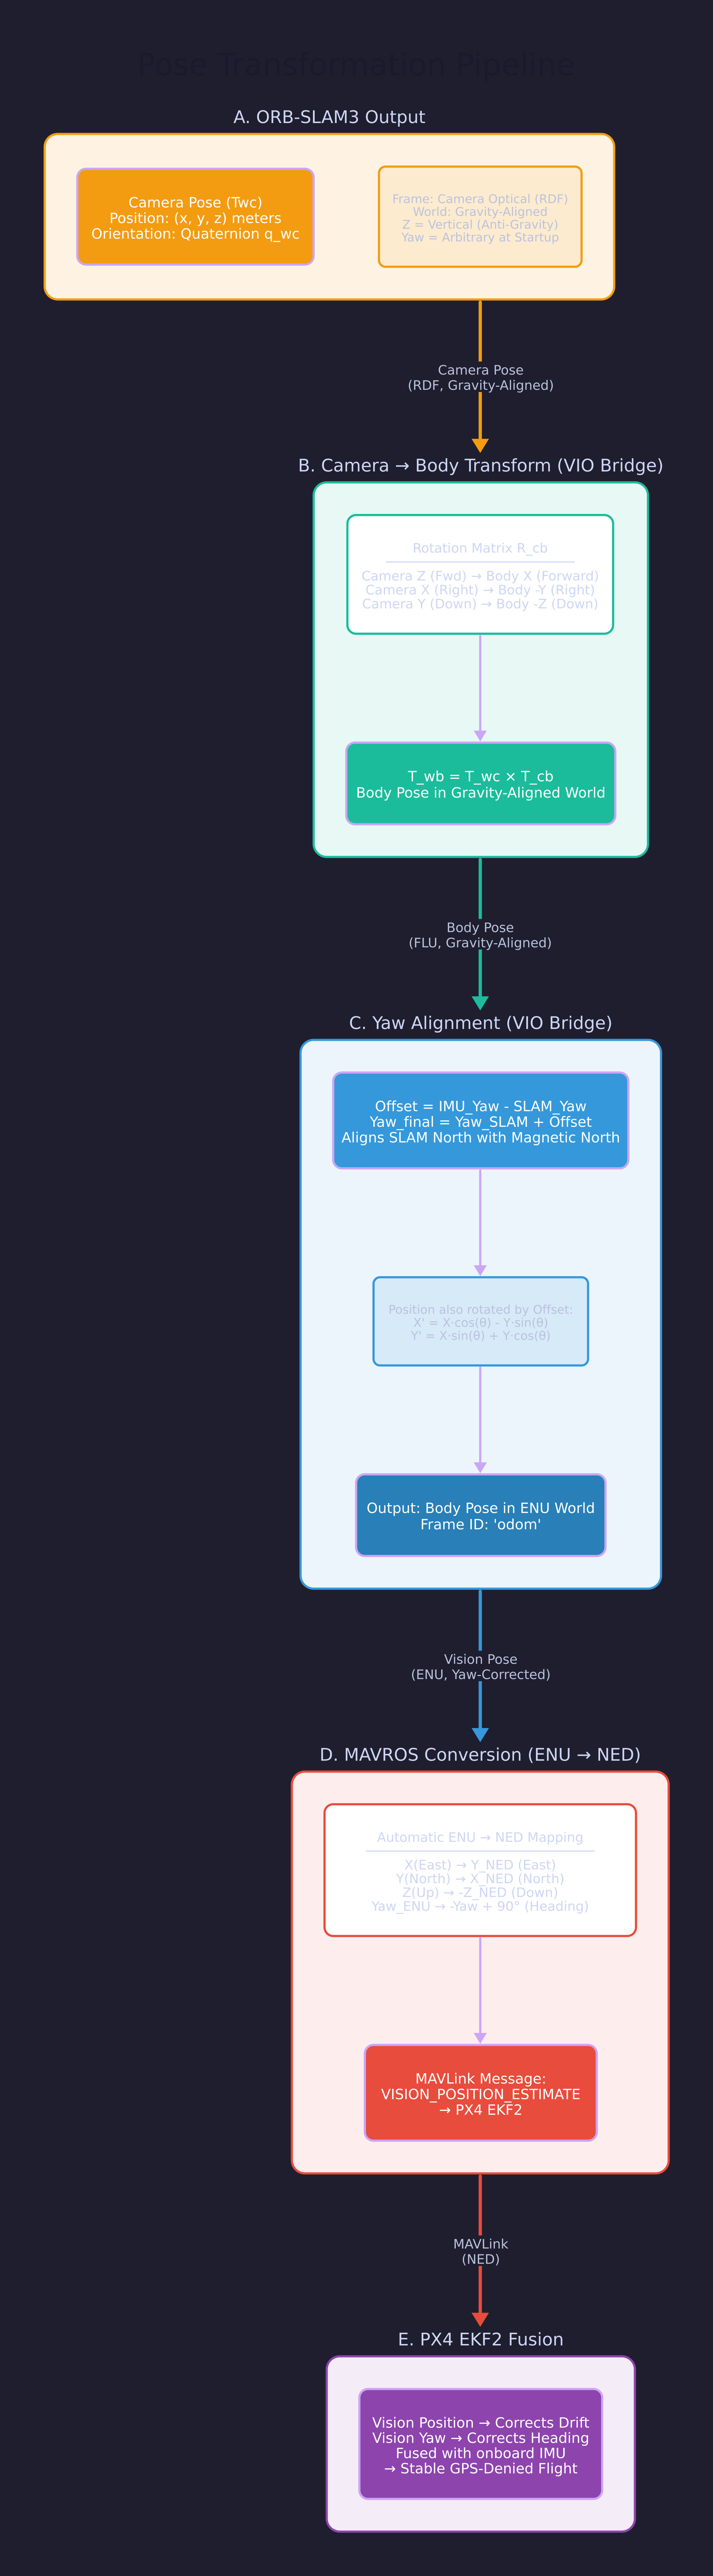
\includegraphics[width=\linewidth,height=0.75\textheight,keepaspectratio]{images/03_pose_pipeline.jpg}
    \caption{Pose Transformation Pipeline}
    \label{fig:pose_transformation}
\end{figure}

\noindent\textbf{ENU $\rightarrow$ NED Conversion (MAVROS):} MAVROS converts the incoming ENU vision pose into the PX4-friendly NED convention as follows:
\begin{itemize}
    \item $X_{\text{NED}} = Y_{\text{ENU}}$ (North)
    \item $Y_{\text{NED}} = X_{\text{ENU}}$ (East)
    \item $Z_{\text{NED}} = -Z_{\text{ENU}}$ (Down)
    \item $\textit{Yaw}_{\text{NED}} = -\textit{Yaw}_{\text{ENU}} + 90^\circ$
\end{itemize}

\begin{table}[H]
\centering
\scriptsize % reduces font size
\caption{PX4 EKF2 Parameters for Vision Fusion}
\resizebox{\textwidth}{!}{%
\begin{tabular}{|p{3.6cm}|p{2.2cm}|p{9.8cm}|}
\hline \textbf{Parameter} & \textbf{Value} & \textbf{Description} \\
\hline EKF2\_EV\_CTRL & 15 & Enable Vision Position, Yaw, Velocity, and Height fusion \\
\hline EKF2\_HGT\_REF & 3 & Set height reference to Vision \\
\hline EKF2\_GPS\_CTRL & 0 & Disable GPS fusion (indoor operation) \\
\hline EKF2\_EV\_DELAY & 50\,ms & Vision processing latency compensation \\
\hline EKF2\_EVP\_NOISE & 0.1 & Vision position noise (confidence) \\
\hline EKF2\_EVA\_NOISE & 0.1 & Vision angle noise (confidence) \\
\hline EKF2\_EV\_POS\_X/Y/Z & 0.0 & Camera-to-IMU offset (measure physically) \\
\hline
\end{tabular}}
\label{tab:px4_ekf2_params_vision}
\end{table}

\subsection{Coordinate Systems and Transformations}
Correct coordinate frame handling is the single most critical aspect of the VIO integration. The system uses four distinct coordinate frames, each with a specific convention. The transformation pipeline flows as: Camera Optical (RDF) $\rightarrow$ [${R}_{cb}$ rotation] $\rightarrow$ Body (FLU) $\rightarrow$ [Yaw correction] $\rightarrow$ World (ENU) $\rightarrow$ [MAVROS auto-conversion] $\rightarrow$ PX4 (NED) $\rightarrow$ [EKF2 fusion] $\rightarrow$ Stable Flight.

\begin{figure}[!ht]
    \centering
    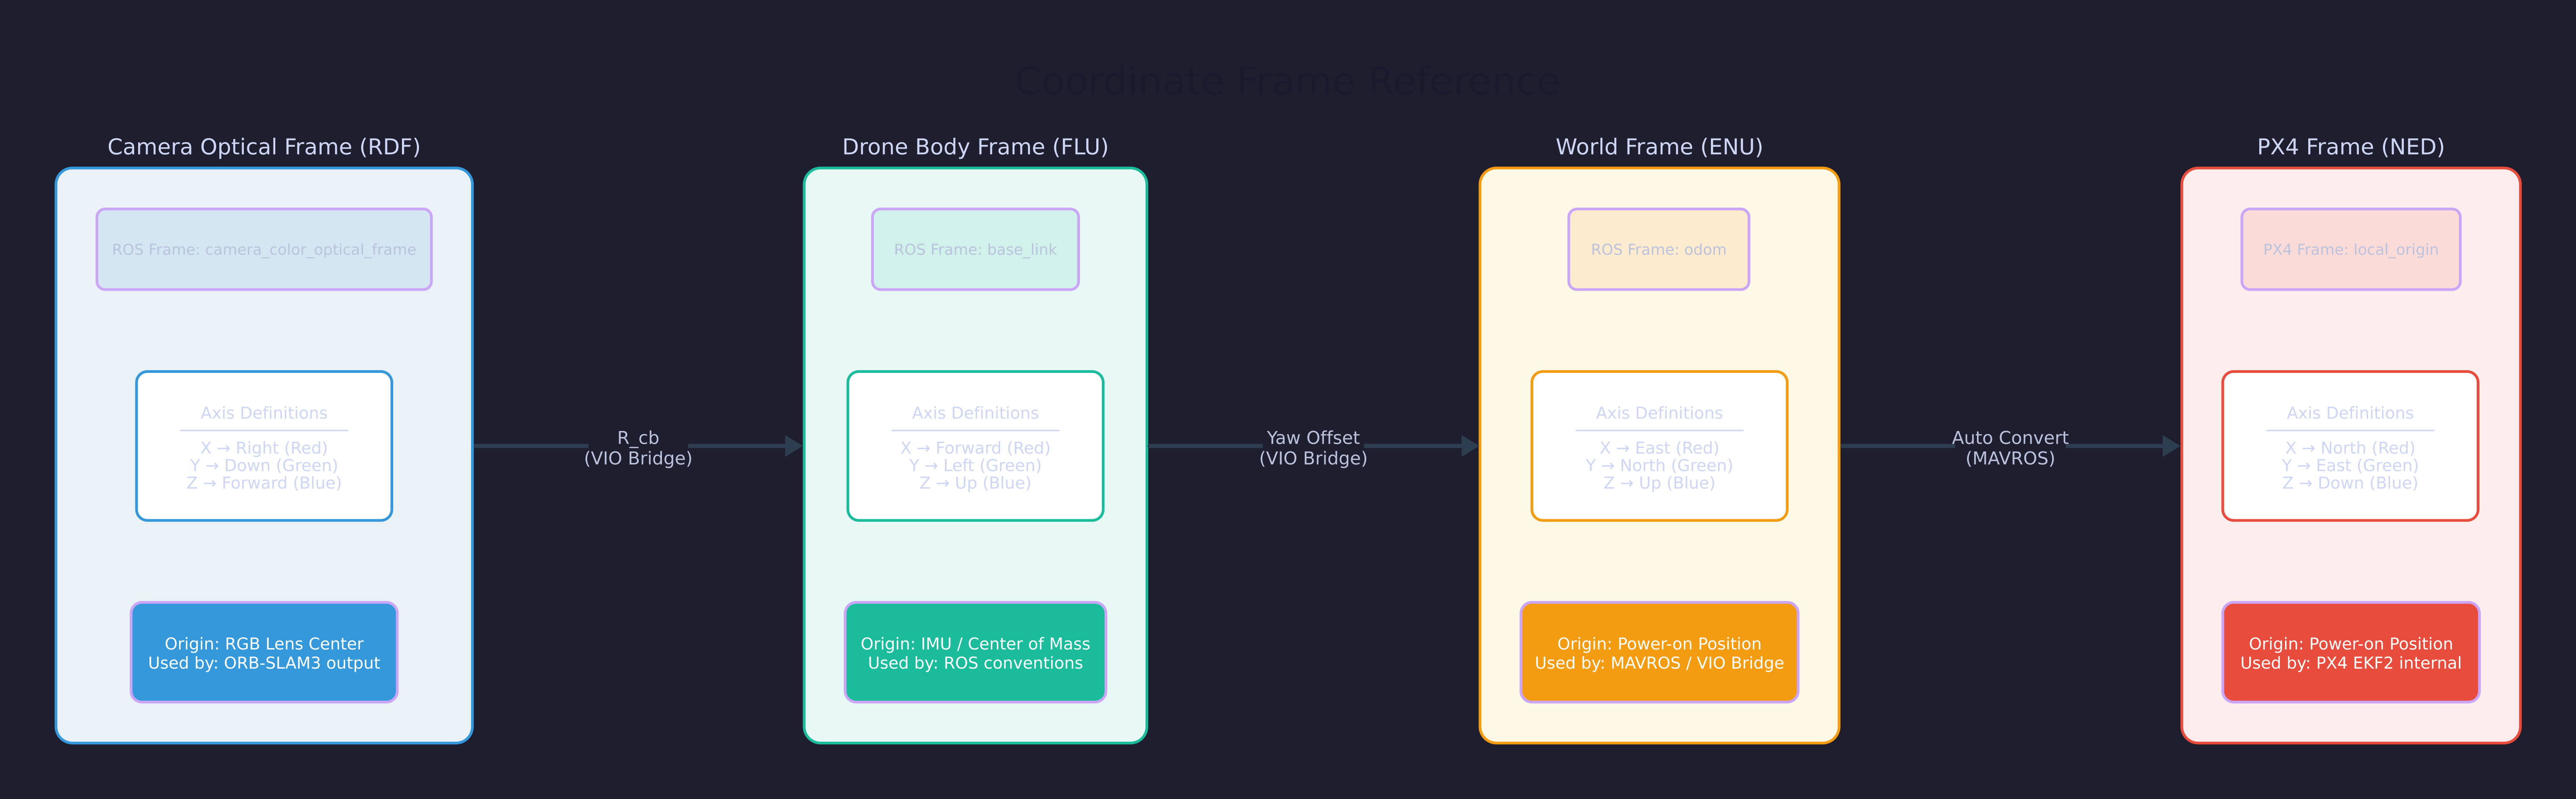
\includegraphics[width=\linewidth,height=0.75\textheight,keepaspectratio]{images/04_coordinate_frames.jpg}
    \caption{Coordinate Frames}
    \label{fig:coordinate_frames}
\end{figure}

\begin{table}[H]
\centering
\scriptsize % reduces font size
\caption{Coordinate Frames Used in the VIO Pipeline}
\resizebox{\textwidth}{!}{%
\begin{tabular}{|p{2.8cm}|p{1.6cm}|p{2.6cm}|p{1.7cm}|p{1.7cm}|p{1.7cm}|p{3.4cm}|}
\hline \textbf{Frame} & \textbf{Convention} & \textbf{ROS Frame ID} & \textbf{X Axis} & \textbf{Y Axis} & \textbf{Z Axis} & \textbf{Used By} \\
\hline Camera Optical & RDF & \texttt{camera\_link} & Right & Down & Forward & ORB-SLAM3 \\
\hline Drone Body & FLU & \texttt{base\_link} & Forward & Left & Up & ROS~2 / VIO Bridge \\
\hline World & ENU & \texttt{odom} & East & North & Up & MAVROS \\
\hline PX4 Internal & NED & \texttt{local\_origin} & North & East & Down & Pixhawk~6X Pro \\
\hline
\end{tabular}}
\label{tab:coordinate_frames}
\end{table}

\subsection{Sensor Calibration}
Accurate calibration is essential for SLAM performance. The following calibration procedures were performed:

\begin{table}[H]
\centering
\scriptsize % reduces font size
\caption{Sensor Calibration Procedures}
\resizebox{\textwidth}{!}{%
\begin{tabular}{|p{3.0cm}|p{6.5cm}|p{7.0cm}|}
\hline \textbf{Procedure} & \textbf{Method} & \textbf{Purpose} \\
\hline Camera Intrinsics & Extracted from \texttt{/camera/color/camera\_info} topic (factory calibration from Orbbec SDK). Verified with checkerboard pattern. & Provides focal lengths (fx=606.96, fy=607.11), principal point (cx=637.73, cy=392.85), and distortion coefficients for accurate feature localization. \\
\hline IMU-Camera Extrinsics & Derived from the static TF between \texttt{camera\_gyro\_optical\_frame} and \texttt{camera\_color\_optical\_frame}. Translation offset of 25\,mm along X-axis. & Defines the rigid 6-DOF transformation ($T_{bc}$) between the IMU and the camera, allowing ORB-SLAM3 to correctly fuse inertial and visual data. \\
\hline IMU Noise Parameters & Empirically tuned --- gyroscope noise: $2.0 \times 10^{-2}$\,rad/s/$\sqrt{\text{Hz}}$, accelerometer noise: $2.0 \times 10^{-1}$\,m/s$^{2}$/$\sqrt{\text{Hz}}$. Values set higher than datasheet specifications. & Deliberately inflated noise values improve initialization stability and prevent the optimizer from trusting noisy consumer-grade IMU data too heavily. \\
\hline
\end{tabular}}
\label{tab:sensor_calibration_procedures}
\end{table}


\subsection{Unified Launch System}
A unified ROS 2 launch file (\texttt{vio\_system.launch.py}) orchestrates the startup of all four nodes with staggered timing to ensure proper initialization order and data availability:
\begin{figure}[!ht]
    \centering
    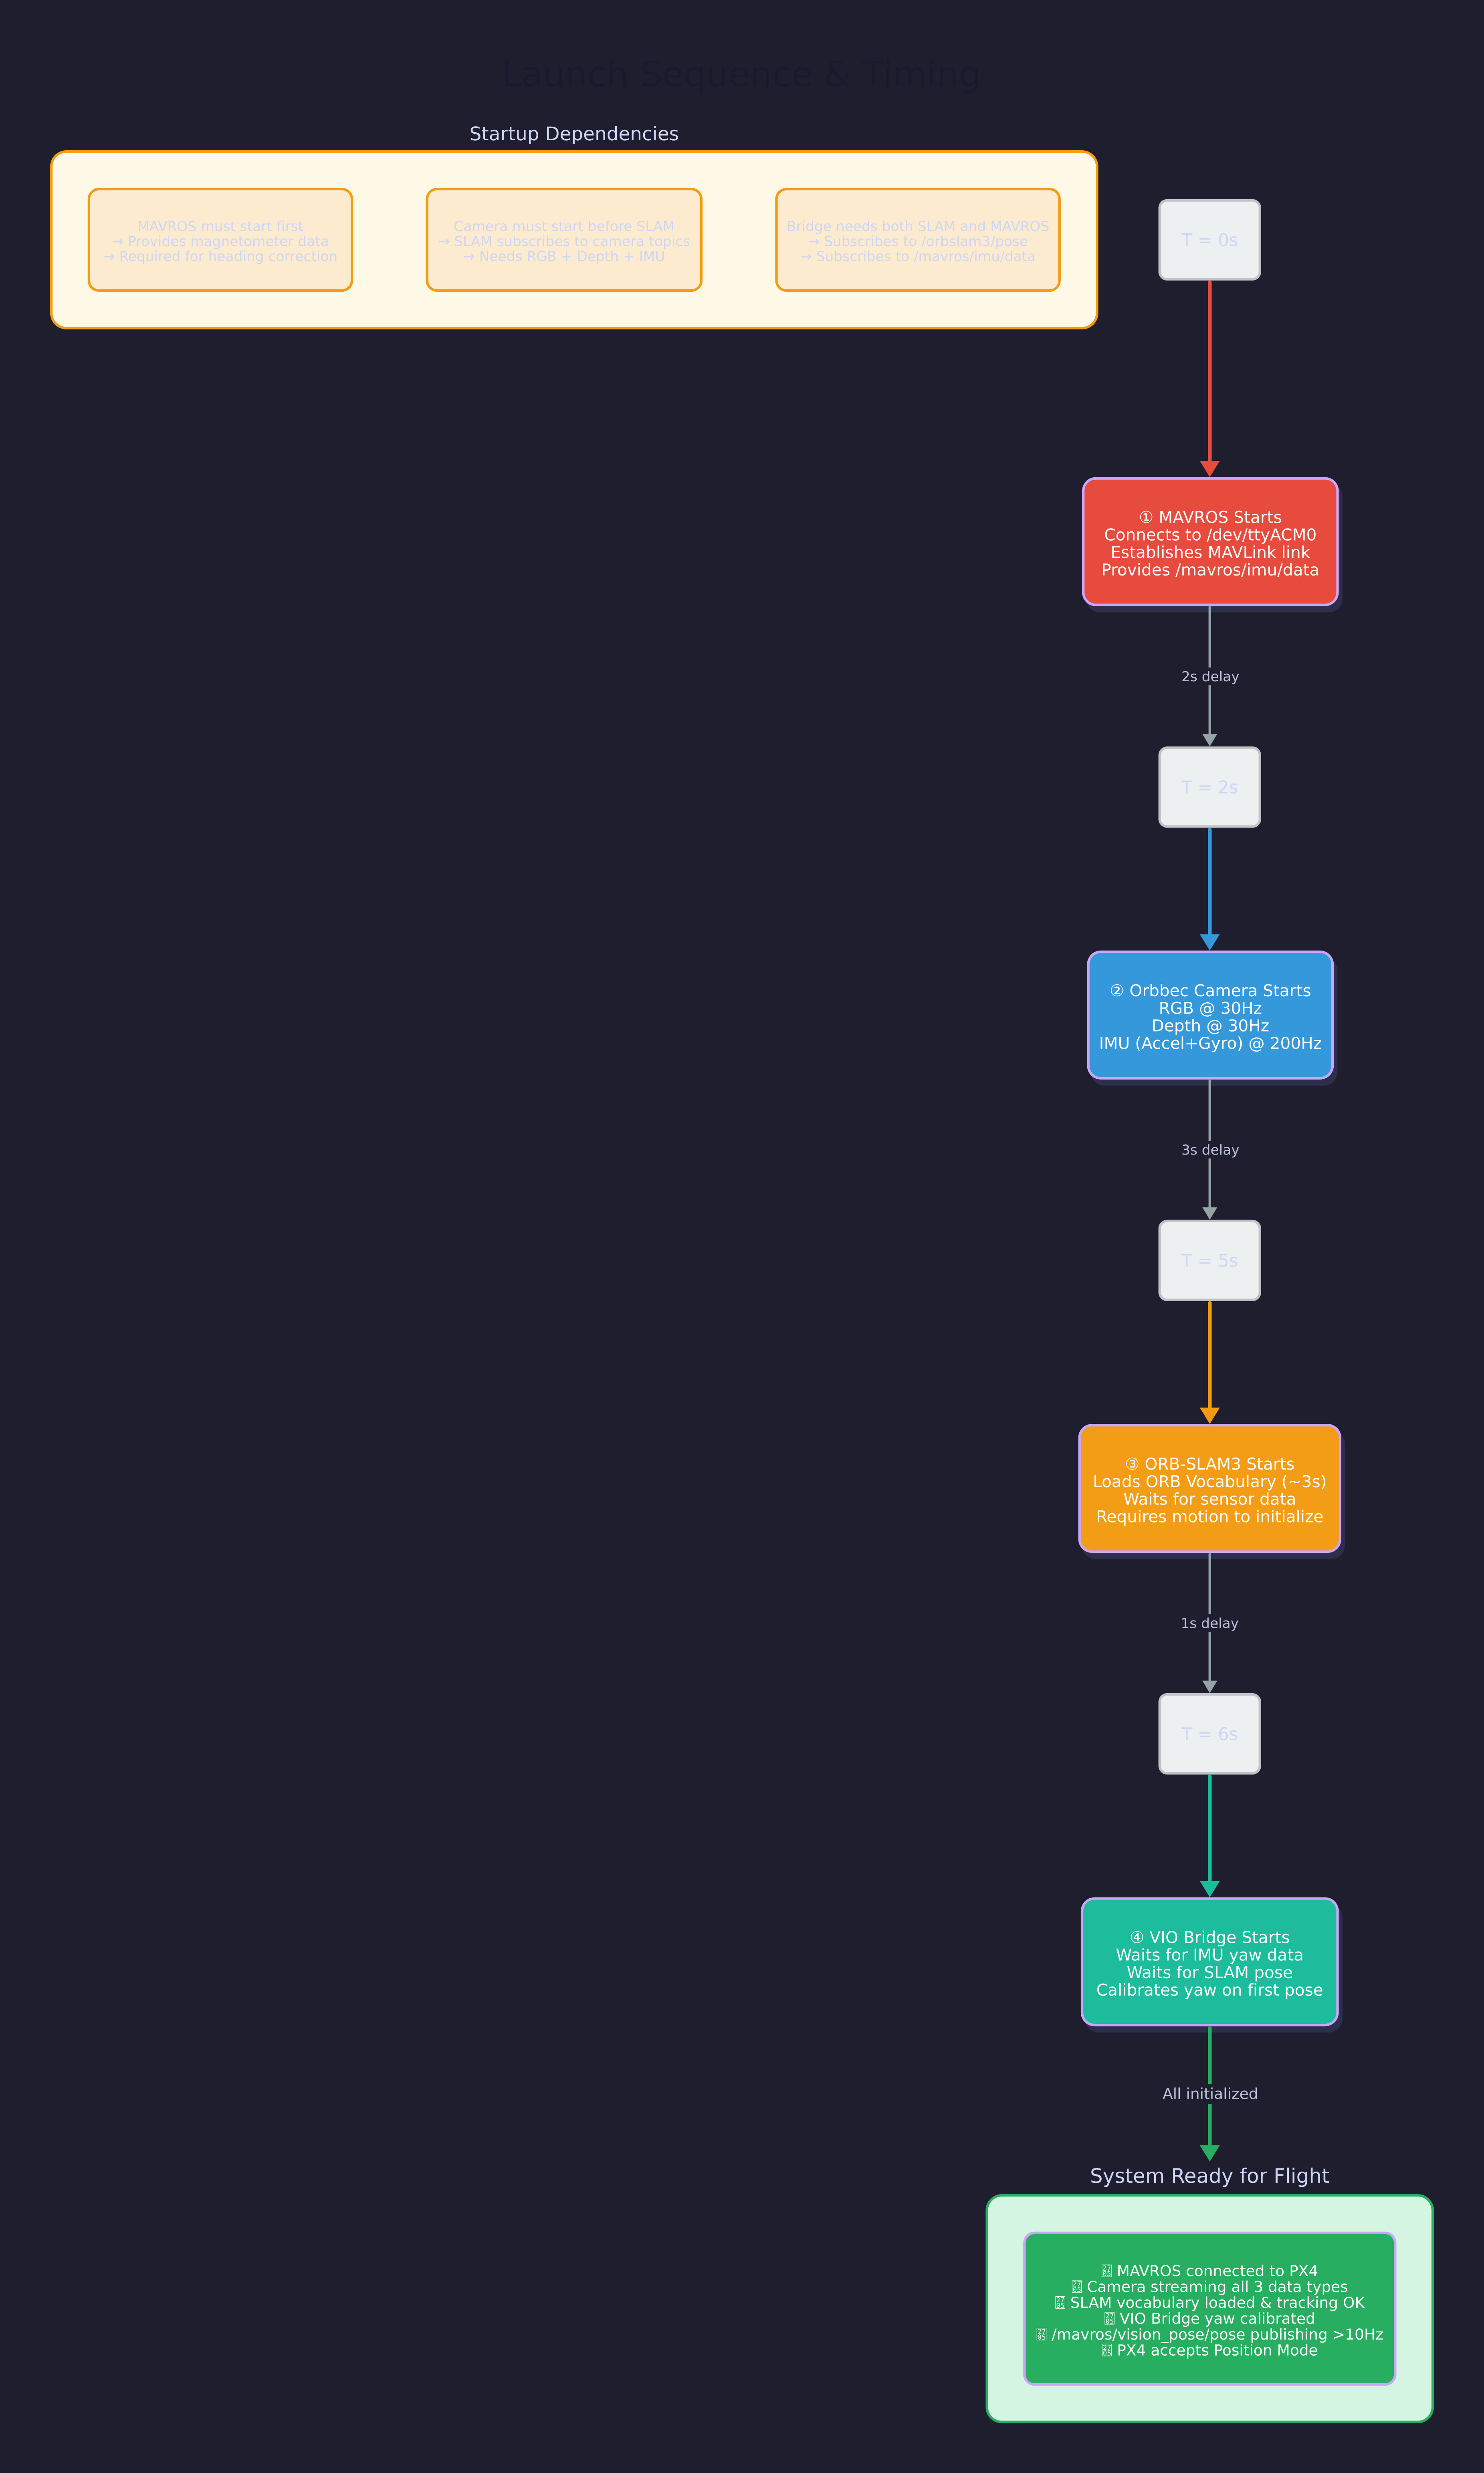
\includegraphics[width=\linewidth,height=0.75\textheight,keepaspectratio]{images/07_launch_sequence.jpg}
    \caption{Launch Sequence}
    \label{fig:launch_sequence}
\end{figure}
\begin{table}[H]
\centering
\scriptsize % reduces font size
\caption{Staggered Launch Schedule for VIO System Nodes}
\resizebox{\textwidth}{!}{%
\begin{tabular}{|p{2.0cm}|p{3.0cm}|p{9.2cm}|p{4.0cm}|}
\hline \textbf{Delay} & \textbf{Node} & \textbf{Reason} & \textbf{Ready Signal} \\
\hline T = 0\,s & MAVROS & Starts first --- must provide magnetometer data to VIO Bridge for heading correction & FCU connection established \\
\hline T = 2\,s & Orbbec Camera & Camera topics must be available before ORB-SLAM3 subscribes & Image and IMU topics publishing \\
\hline T = 5\,s & ORB-SLAM3 & Needs $\sim$3\,s to load vocabulary file (\texttt{ORBvoc.txt}); requires camera data already flowing & ``Vocabulary loaded'' log message \\
\hline T = 6\,s & VIO Bridge & Needs both SLAM pose and MAVROS IMU to be active & \texttt{/mavros/vision\_pose/pose} publishing $>10$\,Hz \\
\hline
\end{tabular}}
\label{tab:launch_schedule}
\end{table}

The launch file exposes configurable arguments for vocabulary path, ORB-SLAM3 config file, FCU URL, GCS URL, and toggles for the SLAM visualizer and magnetometer correction.
\FloatBarrier
\section{Results and Discussion}

\subsection {Testing and Validation Strategy}
A progressive validation approach was adopted to verify the VIO system from individual components through to integrated flight. Each phase builds confidence before introducing additional complexity.


\begin{table}[H]
\centering
\scriptsize % reduces font size
\caption{Testing and Verification}
\resizebox{\textwidth}{!}{%
\begin{tabular}{|p{2.6cm}|p{8.2cm}|p{5.0cm}|}
\hline \textbf{Phase} & \textbf{Procedure} & \textbf{Purpose} \\
\hline
1.\ Component Verification & Independently verified each ROS~2 node: camera topics publishing at correct rates, ORB-SLAM3 tracking in standalone mode, MAVROS connecting to Pixhawk~6X Pro. & Ensures each component functions correctly in isolation before integration. \\
\hline
2.\ Topic Pipeline Verification & Used \texttt{ros2 topic hz} and \texttt{ros2 topic echo} to verify end-to-end data flow: camera $\rightarrow$ SLAM $\rightarrow$ VIO Bridge $\rightarrow$ MAVROS. Checked message types, frame IDs, and rates. & Confirms the data pipeline is correctly wired with proper topic remapping and QoS settings. \\
\hline
3.\ Frame Transform Validation & Manually moved the camera in known directions (forward, right, up) and verified the output pose moved in the expected ENU direction. Cross-referenced with \texttt{/mavros/imu/data} heading. & Validates the $R_{cb}$ rotation matrix and yaw correction produce physically correct pose output. \\
\hline
4.\ PX4 Fusion Verification & Monitored QGroundControl MAVLink Inspector for \texttt{VISION\_POSITION\_ESTIMATE} messages. Verified EKF2 accepted vision data (no rejection warnings). Checked \texttt{/mavros/local\_position/pose} matched vision input. & Confirms PX4 EKF2 is receiving, accepting, and fusing vision pose data into its state estimate. \\
\hline
5.\ Bench Testing (Props Off) & Complete system powered on the drone, propellers removed. Hand-carried through a trajectory while monitoring RViz2 and QGroundControl. Verified Position Mode could be armed. & End-to-end verification that the pose estimate is stable enough for PX4 to accept Position Mode, without risking hardware. \\
\hline
\end{tabular}}
\label{tab:testing_verification}
\end{table}


\subsection{Performance Metrics (KPIs)}
The following Key Performance Indicators are used to evaluate the VIO system:


\begin{table}[H]
\centering
\scriptsize % reduces font size
\caption{Performance Metrics (KPIs)}
\resizebox{\textwidth}{!}{%
\begin{tabular}{|p{3.2cm}|p{2.6cm}|p{10.0cm}|}
\hline \textbf{Metric} & \textbf{Target} & \textbf{Measurement Method} \\
\hline
Localization Drift & $< 10$ cm & Difference between start and end position after closed-loop trajectory \\
\hline
Pose Publish Rate & $> 10$ Hz (stable) & \texttt{ros2 topic hz /mavros/vision\_pose/pose} \\
\hline
Yaw Drift (corrected) & $< 5^\circ$ sustained & VIO Bridge diagnostic output (average drift over 30-sample window) \\
\hline
System Latency & $< 100$ ms & Timestamp delta between camera frame capture and vision pose publication \\
\hline
SLAM Reset Rate & $< 1$ per minute & VIO Bridge diagnostic reset counter \\
\hline
\end{tabular}}
\label{tab:performance_metrics_kpis}

\end{table}



\subsection{Challenges \& Solutions}
This section summarizes the primary integration challenges encountered and the corresponding mitigations implemented.

\subsubsection{IMU Initialization Failure (\texttt{Not enough motion})}
\paragraph{Problem}
ORB-SLAM3 in Inertial mode requires sufficient translational motion to initialize IMU biases and estimate gravity. The system consistently failed to initialize when stationary.
\paragraph{Solution}
Disabled fast initialization (\texttt{IMU.fastInit=0}) and increased IMU noise parameters to be more tolerant. The operational procedure now requires gently sliding the drone left/right and up/down for 5--10~seconds after startup until tracking initializes.

\subsubsection{SLAM Tracking Loss in Low-Texture Environments}
\paragraph{Problem}
White walls and uniform surfaces cause ORB feature extraction to fail, resulting in \texttt{Fail to track local map} errors.
\paragraph{Solution}
Increased ORB features to 1000 across 8 pyramid levels. Lowered the minimum FAST threshold to 7 for better feature detection in low-contrast regions. Operationally, environments are enriched with textured objects where possible.

\subsubsection{Yaw Misalignment Between SLAM and PX4}
\paragraph{Problem}
SLAM initializes with arbitrary heading (Yaw$=0$), causing PX4 to receive poses that are yaw-rotated relative to its magnetometer heading. This resulted in circular flight patterns instead of straight lines.
\paragraph{Solution}
Implemented automatic yaw correction in the VIO Bridge using the AHRS heading from \texttt{/mavros/imu/data}. The bridge continuously monitors for drift and recalibrates when the average error exceeds $15^\circ$ over 30 samples.

\subsubsection{SLAM Reset Causing Position Jumps}
\paragraph{Problem}
When ORB-SLAM3 loses tracking and re-initializes, the position jumps back to the origin, causing PX4 to command a dangerous correction movement.
\paragraph{Solution}
Implemented reset detection in the VIO Bridge: if the position jumps more than 0.5~m toward the origin, the bridge detects a reset and immediately recalibrates the yaw offset. This prevents a stale offset from compounding the jump with a heading error.

\subsubsection{Coordinate Frame Confusion (RDF vs FLU vs ENU vs NED)}
\paragraph{Problem}
Multiple competing conventions across ORB-SLAM3 (optical/RDF), ROS (FLU/ENU), and PX4 (FRD/NED) caused initial integration failures where moving forward appeared as lateral motion.
\paragraph{Solution}
Created comprehensive frame documentation (\texttt{FRAME\_DETAILS.md}) and D2 diagrams. Derived and validated the $R_{cb}$ rotation matrix through systematic physical testing --- moving in each axis independently and verifying the output direction.

\subsection{Next Steps}
The following tasks are planned for the next phase of development:
\begin{itemize}
    \item \textbf{Tethered Flight Testing:} Perform first powered flights with safety tether to validate pose stability under propeller vibration and real aerodynamic conditions. Tune \texttt{EKF2\_EV\_DELAY} based on measured latency.
    \item \textbf{Free Flight Validation:} Execute closed-loop autonomous trajectories in a GPS-denied indoor environment. Measure actual localization drift and compare against the 10~cm KPI target.
    \item \textbf{Vibration Analysis \& Mitigation:} Characterize propeller-induced vibration effects on the camera and IMU. Implement soft-mounting or filtering if vibration degrades SLAM performance on the Holybro Jetson Pack.
    \item \textbf{Covariance Tuning:} Implement dynamic covariance estimation based on ORB-SLAM3 tracking quality (number of matched features, inlier ratio) to give PX4 better confidence information.
    \item \textbf{GPU Acceleration:} Leverage the Jetson Orin NX's 1024-core Ampere GPU for CUDA-accelerated ORB feature extraction and depth processing, reducing CPU load and improving latency.
    \item \textbf{Autonomous Mission Integration:} Develop waypoint-following and return-to-home capabilities using the VIO pose as the primary navigation source.
    \item \textbf{Performance Benchmarking:} Formal measurement of all KPIs during controlled flight tests, including CPU/GPU/RAM load on the Jetson Orin NX 16GB under sustained operation.
\end{itemize}

\section{Project Management}
\sloppy

\subsection{Project Activity Timeline}

\subsubsection{Phase 1: Problem Formulation and Requirement Analysis}
\paragraph{Status:}Completed
This foundational phase has been successfully concluded, establishing the theoretical framework for the project.
\begin{itemize}
    \item \textbf{Literature Review and Background Research:} A systematic review was conducted covering geometric VINS frameworks (OpenVINS, ORB-SLAM3) and Deep Learning-based approaches (SuperPoint, Deep-UAV SLAM).

    \item \textbf{Gap Identification and Problem Statement:} The research identified critical gaps in existing solutions, specifically regarding performance in low texture, low light environments and the computational demands on edge hardware.
    
    \item \textbf{Requirement Gathering:} Functional requirements for real-time localization and non-functional requirements for low-latency processing were defined, guiding the architectural choices.
    
    \item \textbf{Project Proposal Development:} The formal project proposal, outlining the system architecture (ROS 2 nodes, VIO Bridge) and evaluation metrics (ATE, RPE), was prepared and approved, serving as the blueprint for the current implementation phase.

\end{itemize}

\subsubsection{Phase 2: Resource Gathering}
\paragraph{Status:}Completed
All necessary hardware and software environments have been procured and configured.

\begin{itemize}
    \item \textbf{Model Selection:} After reviewing various algorithms (including OpenVINS and PyCuVSLAM), ORB-SLAM3 was selected as the core visual-inertial odometry framework due to its superior global consistency and support for tightly coupled fusion.

    \item \textbf{Dataset Acquisition:} Obtained benchmark datasets (e.g., EuRoC MAV, KITTI) for algorithm testing and training.

    \item \textbf{Hardware Resource Gathering:} The hardware platform has been finalized and assembled, featuring the specific companion computer (e.g., Jetson Orin/Nano as referenced) and flight controller setup.

    \item \textbf{Tool and Platform Setup:} The software stack has been fully deployed. This includes the configuration of ROS 2 (Humble/Foxy) for inter-process communication, PX4 Autopilot for flight control, and the integration of MAVROS to bridge the high-level VIO data with the low-level flight controller.
\end{itemize}

\subsubsection{Phase 3: Model Evaluation}
\paragraph{Status:}Completed
The selected model has undergone rigorous evaluation to ensure it meets the project's performance criteria.

\begin{itemize}
    \item \textbf{Platform-Based Testing:} ORB-SLAM3 has been implemented and tested within the system architecture. The processing pipeline, including feature extraction and local mapping threads, has been validated.

    \item \textbf{Performance Analysis:}  The system's ability to handle sensor data acquisition and processing has been confirmed. Key configuration parameters for the RGB-D Inertial processing pipeline have been tuned.
\end{itemize}

\subsubsection{Phase 4: Drone Integration}
\paragraph{Status:}Ongoing
The project is currently focused on this critical phase, bridging the gap between software algorithms and physical flight control.

\begin{itemize}
\item \textbf{Drone Assembly and Implementation:} Assemble the drone hardware (frames, motors, sensors, communication modules) and integrate all electronic components. Ensure proper wiring, power distribution, and mechanical stability before software integration.
\item \textbf{Algorithm Implementation:} The VIO Bridge node has been successfully developed to handle frame transformations (Camera Frame to Body Frame) and data conversion between the ROS 2 navigation stack and the PX4 flight
\item \textbf{VINS and Flight Controller Integration:} Interface the VINS output with the drone’s flight control system (e.g., PX4, ArduPilot) so that navigation decisions are directly informed by visual-inertial data.
\item \textbf{Flight Testing:} Conduct a series of indoor and outdoor test flights in different conditions: 
    \begin{itemize}
        \item Low light
        \item High wind
        \item GPS-denied areas
    \end{itemize}
    Record performance metrics and operational stability for further refinement.
\end{itemize}

\subsubsection{Phase 5: Model Improvements and Drone Swarm Exploration}
\paragraph{Status:}Pending
Once a working prototype is validated, efforts shift toward improving robustness and extending functionality to swarm scenarios.

\begin{itemize}
    \item \textbf{Limitation Analysis:}  Currently analyzing flight logs to diagnose critical integration issues, specifically yaw misalignment between the VIO estimate and the flight controller's compass, and coordinate frame discrepancies (FLU vs. NED)
    \item \textbf{System Optimization:} Immediate efforts are focused on resolving SLAM initialization failures caused by lack of motion and mitigating "SLAM Reset" events to ensure continuous, smooth trajectory tracking before autonomous flight.
    \item \textbf{Deep Learning Based Optimizations:} Research is ongoing for Deep Learning based optimizations for ORB-SLAM3 computer vision pipeline to address its limitations in lowlight, low texture environments, and to divide workload between CPU and GPU in the Jetson Orin NX.
\end{itemize}

\subsubsection{Phase 6: Documentation and Dissemination}
\paragraph{Status:}Ongoing
Final phase ensures that all technical, operational, and research details are preserved and communicated effectively.

\begin{itemize}
    \item \textbf{Technical Documentation:}  actively documenting the system architecture, specifically the VIO Bridge internal logic, ROS 2 TF tree transformations, and the hardware wiring diagrams for the Jetson Orin/Pixhawk integration.
    \item \textbf{Demonstration:} Organize a live or recorded demonstration showing the system’s capabilities in real flight and/or swarm scenarios.
    \item \textbf{Research Publications:} Compile results into conference papers or journal articles to share findings with the academic and professional community.
    \item \textbf{Final Reports:} The final project report, research publication (targeting VINS performance in GPS-denied environments), and the live flight demonstration are scheduled for the final phase of the project timeline.
\end{itemize}

\subsection{Task Allocation and Individual Contribution}

The following table details the individual contributions of each team member across the comleted project phases and Task Allocation for Upcoming Project Phases
\begin{table}[H]
\centering
\scriptsize
\caption{Task allocation among team members for all project phases.}
\resizebox{\textwidth}{!}{%
\begin{tabular}{|p{2cm}|p{4.3cm}|p{4.3cm}|p{4.3cm}|}
\hline
\textbf{Phase} & \textbf{Akindu} & \textbf{Tishan} & \textbf{Rashmi} \\
\hline

\textbf{Phase 1: Problem Formulation \& Requirement Analysis} &
\begin{itemize}[leftmargin=*, topsep=0pt, itemsep=0pt, parsep=0pt, partopsep=0pt]
  \item Conducted literature review on Deep Learning VIO
  \item Analyzed limitations of VIO in low light, low texture environments.
\end{itemize} &
\begin{itemize}[leftmargin=*, topsep=0pt, itemsep=0pt, parsep=0pt, partopsep=0pt]
  \item Reviewed UAV hardware constraints and GPS-denied navigation challenges.
  \item Specified hardware requirements (Jetson Orin NX, Pixhawk).
\end{itemize} &
\begin{itemize}[leftmargin=*, topsep=0pt, itemsep=0pt, parsep=0pt, partopsep=0pt]
  \item Defined the Problem Statement regarding urban canyon navigation.
  \item Conducted literature review on Geometric VINS (OpenVINS, ORB-SLAM3).
\end{itemize} \\
\hline

\textbf{Phase 2: Resource Gathering} &
\begin{itemize}[leftmargin=*, topsep=0pt, itemsep=0pt, parsep=0pt, partopsep=0pt]
  \item Creating a Github organization to host codebase.
  \item Set up initial software environments and dependencies
\end{itemize} &
\begin{itemize}[leftmargin=*, topsep=0pt, itemsep=0pt, parsep=0pt, partopsep=0pt]
  \item Procure, assemble, and calibrate all hardware components including cameras, IMUs, and embedded computers
  \item Set up the development environment in Jetson Orin NX
\end{itemize} &
\begin{itemize}[leftmargin=*, topsep=0pt, itemsep=0pt, parsep=0pt, partopsep=0pt]
  \item assisted in camera calibration protocols.
  \item Prepared dataset tools for benchmarking.
\end{itemize} \\
\hline

\textbf{Phase 3: Model Evaluation} &
\begin{itemize}[leftmargin=*, topsep=0pt, itemsep=0pt, parsep=0pt, partopsep=0pt]
  \item Evaluated ORB-SLAM3, pycuvslam
  \item Created a ROS2 Wrapper for PyCuVSLAM
\end{itemize} &
\begin{itemize}[leftmargin=*, topsep=0pt, itemsep=0pt, parsep=0pt, partopsep=0pt]
  \item Deployed ORB-SLAM3 node within the ROS 2 framework.
  \item Optimized the RGB-D processing pipeline.
\end{itemize} &
\begin{itemize}[leftmargin=*, topsep=0pt, itemsep=0pt, parsep=0pt, partopsep=0pt]
  \item Evaluated openVINS and Quallcomm qVIO using an exsisting drone
  \item Evaluated camera models and stereo and mono setups
\end{itemize} \\
\hline

\textbf{Phase 4: Drone Integration} &
\begin{itemize}[leftmargin=*, topsep=0pt, itemsep=0pt, parsep=0pt, partopsep=0pt]
  \item Conducting indoor flight tests and manual-to-autonomous switching.
\end{itemize} &
\begin{itemize}[leftmargin=*, topsep=0pt, itemsep=0pt, parsep=0pt, partopsep=0pt]
  \item Developed the VIO Bridge node for ROS 2 $\leftrightarrow$ PX4 communication
  \item Implementing Coordinate Frame Transformations (RDF to FLU).
\end{itemize} &
\begin{itemize}[leftmargin=*, topsep=0pt, itemsep=0pt, parsep=0pt, partopsep=0pt]
  \item Integrating Marker-based localization (ArUco/AprilTags) for drift correction.
\end{itemize} \\
\hline

\textbf{Phase 5: Model Improvement \& Swarm Exploration} &
\begin{itemize}[leftmargin=*, topsep=0pt, itemsep=0pt, parsep=0pt, partopsep=0pt]
  \item Augmenting ORB-SLAM3 computer vision pipeline with deep learning based components and testing
\end{itemize} &
\begin{itemize}[leftmargin=*, topsep=0pt, itemsep=0pt, parsep=0pt, partopsep=0pt]
  \item Integrating Enhaced ORBSLAM3 with the drone and HITL Testing
\end{itemize} &
\begin{itemize}[leftmargin=*, topsep=0pt, itemsep=0pt, parsep=0pt, partopsep=0pt]
  \item Implementing algorithmic fixes for initialization failures (stationary start).
\end{itemize} \\
\hline

\textbf{Phase 6: Documentation \& Dissemination} &
\begin{itemize}[leftmargin=*, topsep=0pt, itemsep=0pt, parsep=0pt, partopsep=0pt]
  \item Preparing and Maintaining documentation in repositories
  \item Producing the Video Demonstration of the flight tests.
\end{itemize} &
\begin{itemize}[leftmargin=*, topsep=0pt, itemsep=0pt, parsep=0pt, partopsep=0pt]
  \item Documenting Software Architecture, VIO Bridge logic, and API references.
  \item Creating Hardware Integration Manuals and wiring diagrams.
\end{itemize} &
\begin{itemize}[leftmargin=*, topsep=0pt, itemsep=0pt, parsep=0pt, partopsep=0pt]
  \item Compiling Documentation
  \item Organize demonstration materials
  \item Prepare publications for academic dissemination
\end{itemize} \\
\hline

\end{tabular}}
\end{table}


\subsection{Summary}
% Shown in the following Table is a summary of project activities in each phase of the project.
% \begin{table}[H]
% \centering
% \small
% \begin{tabular}{|p{3cm}|p{5.5cm}|p{5.5cm}|}
% \hline
% \textbf{Phase} & \textbf{Main Focus} & \textbf{Expected Outcomes} \\ \hline
% 1. Problem Formulation & Define problem, requirements, proposal & Clear problem statement, project proposal, defined scope \\ \hline
% 2. Resource Gathering & Collect models, datasets, platforms & Ready-to-use algorithms, datasets, and simulation environments \\ \hline
% 3. Model Evaluation & Test and compare VINS models & Performance metrics, best model selected \\ \hline
% 4. Drone Integration & Implement and test VINS on hardware & Functional VINS-enabled drone with tested navigation \\ \hline
% 5. Model Improvement \& Swarm Exploration & Optimize system, extend to swarm & Improved robustness, initial swarm coordination results \\ \hline
% 6. Documentation \& Dissemination & Reporting and sharing findings & Technical documentation, publications, final project report \\ \hline
% \end{tabular}
% \caption{Summary of Methodology Phases with Focus and Expected Outcomes.}
% \end{table}

\begin{figure}[H]
    \centering
    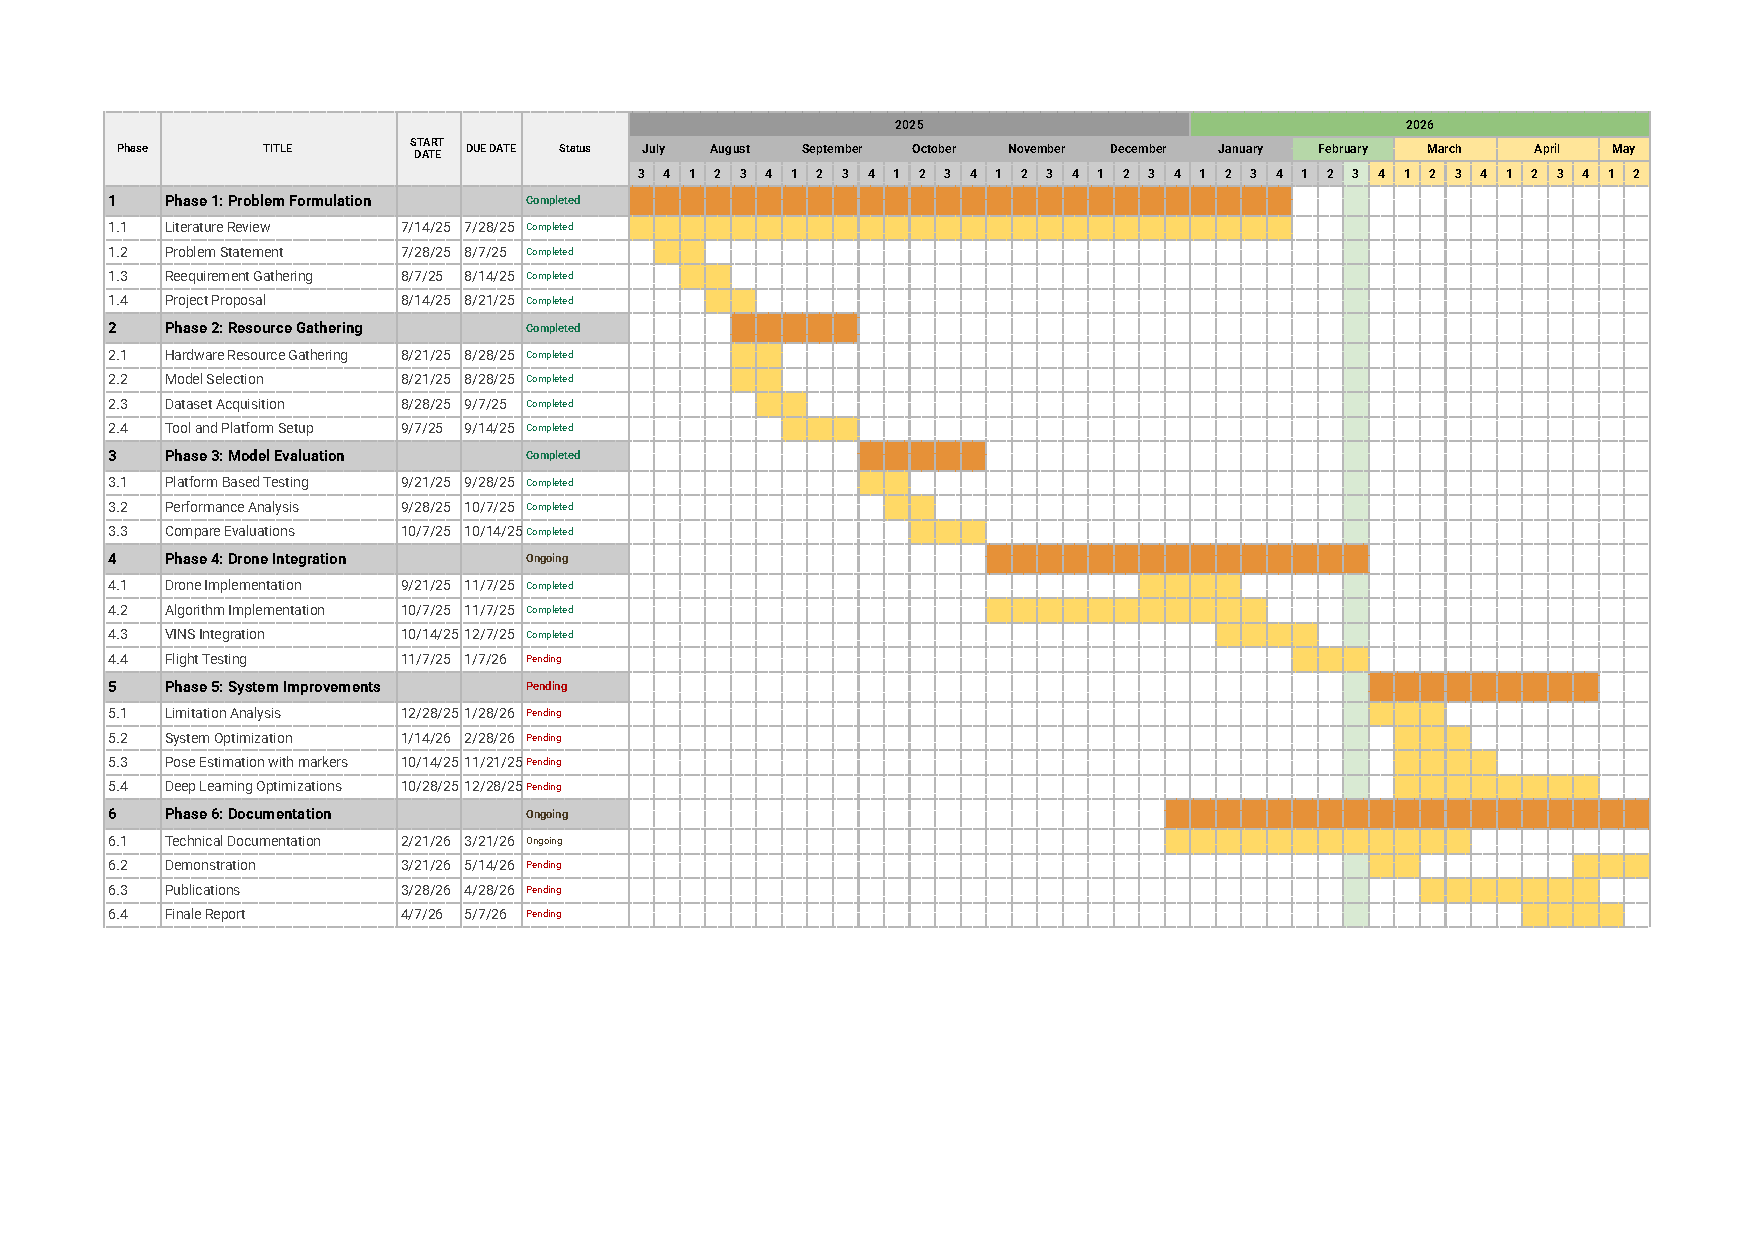
\includegraphics[width=\textwidth, trim=1.6cm 4cm 1.6cm 1.8cm, clip]{images/gantt_chart_2.pdf}
    \caption{Research Timeline}
    \label{fig:gantt_chart}
\end{figure}

\section{Conclusion}
This progress report presented the design and early validation of a Visual--Inertial Odometry (VIO) pipeline intended to enable reliable UAV navigation in GPS-restricted environments. Motivated by the limitations of GNSS in indoor, urban-canyon, and under-canopy scenarios, the work consolidated key VINS concepts and justified a tightly-coupled, optimization-driven approach as the most suitable foundation for robust state estimation under challenging sensing conditions.

Building on these findings, the project implemented a modular ROS~2 architecture that integrates an RGB-D + IMU sensor (Orbbec Gemini~2L), an RGBD-Inertial ORB-SLAM3 back-end, a custom VIO bridge for frame transformation and yaw alignment, and a MAVROS interface that delivers vision-based pose estimates to PX4 for EKF2 fusion. A structured test strategy was defined to verify the system progressively from individual node correctness, to end-to-end topic flow, frame-transform validity, and flight-controller acceptance of \texttt{VISION\_POSITION\_ESTIMATE} messages.

Initial results highlight the main practical challenges of real-world deployment---IMU initialization requirements, tracking degradation in low-texture scenes, yaw inconsistency between SLAM and the flight controller, SLAM reset-induced position discontinuities, and confusion across RDF/FLU/ENU/NED conventions---and document the mitigations introduced in software and operating procedure. These outcomes provide a concrete baseline for subsequent flight testing and quantitative benchmarking against the defined KPIs (drift, pose rate, yaw stability, latency, and reset frequency).

Future work will focus on tethered and free-flight validation in GPS-denied environments, vibration characterization and mitigation, covariance and delay tuning for improved PX4 fusion behavior, and performance optimization (including GPU acceleration on the Jetson platform). Collectively, these steps aim to transition the current integrated prototype into a robust navigation module that can support higher-level autonomy tasks such as waypoint following and, ultimately, multi-UAV coordination in complex real-world missions.

\section{References}
\begingroup
\noindent
\printbibliography[heading=none]
\endgroup
\end{document}